\documentclass[abstract=on,10pt,a4paper,bibliography=totocnumbered]{article}
\usepackage[paper=a4paper,left=35mm,right=35mm,top=25mm,bottom=30mm]{geometry}
\usepackage[doublespacing]{setspace}
\usepackage[english]{babel}
\usepackage[utf8]{inputenc}
\usepackage[T1]{fontenc}
\usepackage{amsmath}
\usepackage{colortbl}
\usepackage{amsfonts}
\usepackage{amssymb}
\usepackage{gensymb}
\usepackage{textcomp}
\usepackage{graphicx}
\usepackage{tikz}
\usepackage{enumerate}
\usepackage{enumitem}
\usepackage{subcaption}
\usepackage{booktabs}
\usepackage[hidelinks]{hyperref}
\usepackage[nameinlink]{cleveref}
\usepackage{multirow}
\usepackage{arydshln}
\usepackage[flushleft]{threeparttable}
\usepackage[nomarkers, nolists]{endfloat}
\usepackage{scalerel}
\usepackage{makecell}
\usepackage{ifthen}
\usepackage{tikz}
\usepackage{lineno}
\usetikzlibrary{svg.path}

%------------------------------------------------------------------------------
%  Bibtex vs Biblatex
%------------------------------------------------------------------------------
% While bibtex is very nice to use, it's insanely slow. I therefore work with
% bibtex until the final stage. Set the value below to "true" or "false" to pick
% which one should be used.
\newboolean{usebiblatex}
\setboolean{usebiblatex}{false}

% Depending on the question, the commands below will prepare the document
% accordingly
\ifthenelse{\boolean{usebiblatex}}{
  %-----------------------------------------------------------------------------
  %  If using biblatex
  %-----------------------------------------------------------------------------
  % Load required packages and refer to correct bibliography
  \usepackage{csquotes}
  \usepackage[
      backend=biber
    , style=apa          % To display Author-year in the text
    , natbib=true        % Necessary to use citep, etc.
    , hyperref=true      % To have clickable links in the references
    , useeditor=false    % Don't add editor to publications
    , sorting=ynt        % Sort by year, name, and title
    , uniquename=false   % Avoid that initials are put
  ]{biblatex}
  \addbibresource{Literature.bib}

  % To include author in link
  \DeclareFieldFormat{citehyperref}{%
  \DeclareFieldAlias{bibhyperref}{noformat}% Avoid nested links
  \bibhyperref{#1}}
  \DeclareFieldFormat{textcitehyperref}{%
  \DeclareFieldAlias{bibhyperref}{noformat}% Avoid nested links
  \bibhyperref{%
    #1%
    \ifbool{cbx:parens}
      {\bibcloseparen\global\boolfalse{cbx:parens}}
      {}}}
  \savebibmacro{cite}
  \savebibmacro{textcite}
  \renewbibmacro*{cite}{%
    \printtext[citehyperref]{%
      \restorebibmacro{cite}%
      \usebibmacro{cite}}}
  \renewbibmacro*{textcite}{%
    \ifboolexpr{
      ( not test {\iffieldundef{prenote}} and
        test {\ifnumequal{\value{citecount}}{1}} )
      or
      ( not test {\iffieldundef{postnote}} and
        test {\ifnumequal{\value{citecount}}{\value{citetotal}}} )
    }
      {\DeclareFieldAlias{textcitehyperref}{noformat}}
      {}%
    \printtext[textcitehyperref]{%
      \restorebibmacro{textcite}%
      \usebibmacro{textcite}}}

  % Remove editor form everything but books
  \AtEveryBibitem{%
   \ifentrytype{book}{}{%
    \clearname{editor}
   }
  }
}{
  %-----------------------------------------------------------------------------
  %  If using bibtex
  %-----------------------------------------------------------------------------
  % Load required packages and select citation style
  \usepackage[round]{natbib}
  \bibliographystyle{apalike}
}

%------------------------------------------------------------------------------
%	Some Styling
%------------------------------------------------------------------------------
% Link colors
\definecolor{linkcolor}{HTML}{000000}
\hypersetup{
  colorlinks = true,
  linkcolor  = linkcolor,
  urlcolor   = linkcolor,
  citecolor  = linkcolor,
}

% Changing the style of captions in figures etc.
\captionsetup{labelfont=bf, format=plain, font=small}

% Change how equations are referenced
\renewcommand{\theequation}{Equation \arabic{equation}}%

% Avoid skip when including text from external .tex file
\newcommand{\inputy}[1]{\input{#1}\unskip}

% For supplementary material
\newcommand{\beginappendix}{%
  \setcounter{table}{0}
  \renewcommand{\thetable}{S\arabic{table}}%
  \setcounter{figure}{0}
  \renewcommand{\thefigure}{S\arabic{figure}}%
  \setcounter{equation}{0}
  \renewcommand{\theequation}{Equation S\arabic{equation}}%
  \setcounter{section}{0}
  \renewcommand{\thesection}{A.\arabic{section}}%
}

%------------------------------------------------------------------------------
%  ORCID
%------------------------------------------------------------------------------
% Creating some TikZ styles
\tikzset{
  nonterminal/.style = {rectangle
    , minimum size = 6mm
    , very thick
    , draw = black!
  }
}

% Create the ORCID logo
\definecolor{orcidlogocol}{HTML}{A6CE39}
\tikzset{
  orcidlogo/.pic={
    \fill[orcidlogocol]
      svg{M256,128c0,70.7-57.3,128-128,128C57.3,256,0,198.7,0,128C0,57.3,57.3
        ,0,128,0C198.7,0,256,57.3,256,128z};
    \fill[white]
      svg{M86.3,186.2H70.9V79.1h15.4v48.4V186.2z}
      svg{M108.9,79.1h41.6c39.6,0,57,28.3,57,53.6c0,27.5-21.5,53.6-56.8
        ,53.6h-41.8V79.1z M124.3,172.4h24.5c34.9,0,42.9-26.5
        ,42.9-39.7c0-21.5-13.7-39.7-43.7-39.7h-23.7V172.4z}
      svg{M88.7,56.8c0,5.5-4.5,10.1-10.1,10.1c-5.6,0-10.1-4.6-10.1-10.1c0-5.6
      ,4.5-10.1,10.1-10.1C84.2,46.7,88.7,51.3,88.7,56.8z};
  }
}

% Command to create the ORCID
\newcommand\orcid[1]{\href{https://orcid.org/#1}{\mbox{\scalerel*{

\begin{tikzpicture}[yscale=-1,transform shape]
  \pic{orcidlogo};
\end{tikzpicture}
}{|}}}}

%------------------------------------------------------------------------------
%	Titlepage: Header
%------------------------------------------------------------------------------
\title{The Effects of Increasing Seasonal Dynamism when Predicting Connectivity:
Advantages or Unnecessary Complications?}

% List of Authors
\author{
  David D. Hofmann\textsuperscript{1,2,\S} \orcid{0000-0003-3477-4365} \and
  Dominik M. Behr\textsuperscript{1,2} \orcid{0000-0001-7378-8538} \and
  John W. McNutt\textsuperscript{2} \and
  Arpat Ozgul\textsuperscript{1, 2} \orcid{0000-0001-7477-2642} \and
  Gabriele Cozzi\textsuperscript{1,2} \orcid{0000-0002-1744-1940}
}

% Reduce spacing between authors
\makeatletter
\def\and{%
  \end{tabular}%
  \hskip -0.5em \@plus.17fil\relax
  \begin{tabular}[t]{c}}
\makeatother

% Current Date
% \date{\today}

% And here the masterpiece begins
\begin{document}

% Change page numbering
\pagenumbering{gobble}

% Create Titlepage
\maketitle

%------------------------------------------------------------------------------
%	Titlepage: Additional Info
%------------------------------------------------------------------------------
\begin{flushleft}

\vspace{0.5cm}

\textsuperscript{1} Department of Evolutionary Biology and Environmental
Studies, University of Zurich, Winterthurerstrasse 190, 8057 Zurich,
Switzerland.

\textsuperscript{2} Botswana Predator Conservation Program, Wild Entrust,
Private Bag 13, Maun, Botswana.

\textsuperscript{\S} Corresponding author: \href{mailto://david.hofmann2@uzh.ch}{david.hofmann2@uzh.ch}

\vspace{4cm}

\textbf{Running Title:} Connectivity in Seasonal Landscapes

\vspace{0.5cm}

\textbf{Keywords:} African wild dog, Connectivity, Dispersal, Dynamism,
Individual-based, Lycaon pictus, Okavango Delta, Seasonality

\end{flushleft}

%------------------------------------------------------------------------------
%	Abstract
%------------------------------------------------------------------------------
\newpage
\begin{abstract}

Seasonally changing conditions can drastically alter landscape connectivity.
Nevertheless, most connectivity studies ignore seasonal dynamism and instead
employ a static set of spatial covariates and assume their focal species to
exhibit a static set of preferences. Ignoring seasonality may, however, mask
important ecological features and processes, thus resulting in poor agreement
between predicted and observed movements and a misrepresentation of
connectivity.

We present a simple framework highlighting that seasonality may enter a
connectivity analysis at three distinct stages, namely when (1) extracting
spatial covariates for model fitting, (2) when fitting the selection model, and
(3) when making predictions from the fitted model. In combination, this provides
six possible configurations that differ in terms of the seasonal dynamism they
encapsulate.

Capitalizing on natural seasonal fluctuations of the Okavango Delta in northern
Botswana and on GPS data collected on dispersing African wild dogs
(\textit{Lycaon pictus}) across different seasons, we investigate the degree to
which a better representation of seasonal dynamism improves our ability to
predict connectivity. For this, we fit integrated step-selection functions and
predict connectivity using an individual-based dispersal simulation while
explicitly considering seasonal dynamism in both environmental covariates and
the species' preferences.  Using a rigorous cross-validation procedure, we
compare the predictive model performance under each of the six proposed
configurations. While we expected that an increasing degree of seasonal dynamism
would lead to improved predictions, we were particularly interested in
identifying at which stage the inclusion of seasonality provides the biggest
benefits.

We show that, for our study system, improvements in predictive performance by
incorporating seasonal dynamism were moderate. In fact, incorporating
seasonality only improved predictions when an overly simplistic movement model
was assumed. Upon fitting a more complex model, the benefits of accounting for
seasonality vanished, resulting in imperceptible performance differences.
Despite this, patterns of connectivity as obtained from dispersal simulations
revealed marked differences between the most static and most dynamic
configurations. Most notably, connectivity was more homogeneously distributed
throughout the study area when seasonality was taken into account, suggesting
the existence of seasonal stepping stones that facilitate dispersal into
otherwise inaccessible areas.

Besides a better understanding of the importance of dynamic connectivity, our
results also provide insights into the conservation needs of the endangered
African wild dog.

\end{abstract}

%------------------------------------------------------------------------------
%	Main Text
%------------------------------------------------------------------------------
\newpage

\onehalfspacing
\tableofcontents
\doublespacing

% Change page numbering
\newpage
\pagenumbering{arabic}

% Create linenumbers
\linenumbers
\section{Introduction}
\subsection{Connectivity}

Landscape connectivity is defined as the degree to which the landscape
facilitates or impedes movement among habitat patches \citep{Taylor.1993} and is
a critical prerequisite for maintaining biodiversity \citep{Fahrig.2003}.
Improved connectivity facilitates dispersal \citep{Doerr.2011, Baguette.2013},
which in turn promotes genetic diversity \citep{Perrin.2000, Frankham.2002} and
the colonization of vacant habitats \citep{Hanski.1999, MacArthur.2001}. Due to
its beneficial impacts on metapopulation dynamics, restoring connectivity is
among the most frequently recommended strategies to conserve biodiversity and to
promote resilience against climate change \citep{Heller.2009, Rudnick.2012}.
Quantifying connectivity and identifying critical dispersal corridors have
therefore become critical tasks in conservation science \citep{Heller.2009,
Rudnick.2012, Keeley.2019, Hofmann.2021}. One aspect that has received limited
attention in the study of connectivity is the role of seasonality. Yet, seasonal
changes both in the environment and in an animal's propensity to use or avoid
particular habitat types can profoundly impact landscape connectivity
\citep{Zeller.2020a}.

\subsection{Seasonality}

Seasonality can impact functional connectivity through spatio-temporal variation
in the landscape itself, or through temporal variation in species' preferences
towards prevailing conditions \citep{Mui.2017, Simpkins.2017a, Zeller.2020a}. In
ecosystems that experience alternations between wet and dry seasons, for
example, the onset of the rainy season initiates distinct ``green-up'' waves,
which affect the availability of food resources for herbivores and,
subsequently, shape their movements \citep{Merkle.2016}. In its most remarkable
form, the variation in environmental conditions drives herbivore migrations
across massive spatial scales, resulting in short-lived movement corridors
between two otherwise disconnected habitats \citep{Serneels.2001, Naidoo.2016}.
Alternatively, seasonality can affect functional connectivity via temporal
changes in a species' movement and habitat preferences. Amphibians, for
instance, require both aquatic and terrestrial habitats, but their preference
for one over the other heavily depends on the season \citep{Baldwin.2006}.
Although such seasonal intricacies are likely to play a fundamental role in many
ecosystems, they only rarely enter connectivity studies in an explicit manner.
In fact, most connectivity studies represent their study system by a static set
of environmental layers and assume that their focal species exhibits a fixed set
of preferences (e.g., \citealp{Elliot.2014, Abrahms.2017, Brennan.2020}).
However, this may result in biased connectivity estimates and a misallocation of
scarce conservation funds \citep{Osipova.2019, Zeller.2020}. Therefore, a more
dynamic approach to connectivity that acknowledges and renders seasonal
variation has been recommended \citep{Zeller.2020a}.

\subsection{Modeling Functional Connectivity}

Functional connectivity can be estimated using a variety of modeling techniques
\citep{Diniz.2019}, which all comprise four main steps. First, presence data of
the focal species, preferably collected during dispersal (\citealp{Elliot.2014,
Vasudev.2015, Benz.2016}, but see \citealp{Fattebert.2015}), and a set of
spatial covariate layers that are believed or known to be critical determinants
of connectivity are compiled. Second, these data are combined and fed into a
selection model that enables estimating a species selection or avoidance of
environmental features. Popular frameworks for estimating preferences are
case-control designs, where characteristics extracted at observed locations are
contrasted with characteristics extracted at available locations
\citep{Beyer.2010, Fieberg.2010}. This can be achieved using point-selection
functions \citep{Boyce.2002, Manly.2007}, path-selection functions
\citep{Cushman.2010}, and step-selection functions \citep{Fortin.2005,
Thurfjell.2014}. A particularly powerful approach is that of \textit{integrated}
step-selection functions (iSSFs), as it provides an effective means to model
both an animal's habitat-selection and movement capacity \citep{Avgar.2016,
Fieberg.2021}. Third, inferred preferences are used to predict a permeability
surface, which indicates the expected ease or difficulty at which the focal
species can traverse a certain area given the area's environmental
characteristics \citep{Zeller.2012}. Finally, in a fourth step, the permeability
surface serves as an input to a connectivity model that reveals crucial movement
corridors. At present, the most popular connectivity models are least-cost path
analysis \citep{Adriaensen.2003} and circuit theory \citep{McRae.2008}, although
individual-based movement models (IBMMs) have gained some momentum recently
\citep{Kanagaraj.2013, Allen.2016, Hauenstein.2019, Zeller.2020,
UnnithanKumar.2022a, UnnithanKumar.2022, Hofmann.2023}. In particular, some
IBMMs allow estimating connectivity directly via simulated dispersal
trajectories, thus bypassing the generation of a permeability surface
\citep{UnnithanKumar.2022a, Hofmann.2023}.

\subsection{Incorporating Seasonality in Functional Connectivity Models}

Seasonality can enter the connectivity modeling workflow described above in
three distinct stages (\Cref{GraphicalAbstract}). In the first stage, one can
either extract environmental features, such as water and vegetation, from a
static layer (i.e., a single snapshot) or from a time series of layers (i.e., a
sequence of snapshots) that capture seasonal variation across the landscape. The
former approach has historically been the norm (e.g., \citealp{Elliot.2014,
Brennan.2020}), yet advances in remote sensing technologies and a facilitated
access to petabytes of landscape data have opened up new avenues for obtaining
spatial layers at unprecedented spatio-temporal resolutions \citep{Toth.2016,
Rumiano.2020}, such that the representation of study systems via dynamic
covariate layers has become more frequent (e.g., \citealp{Osipova.2019,
Kaszta.2021}). In a second stage, one can assume their focal species to exhibit
a fixed set of preferences across seasons by pooling all presence data, or can
try to account for seasonal changes in preferences by splitting the data
accordingly (e.g., \citealp{Fortin.2005, Manly.2007, Cushman.2010,
Zeller.2020}). \cite{Chetkiewicz.2009}, for instance, partitioned their data by
season to derive seasonal habitat preferences for pumas (\textit{Puma concolor})
and grizzlies (\textit{Ursus arctos}). In a final stage, one can estimate
connectivity for either ``average'' environmental conditions, or utilize
seasonally updated layers to estimate connectivity for distinct seasons. For
connectivity models that rely on permeability surfaces, this implies repeatedly
applying the connectivity model using seasonally updated resistance surfaces
(e.g. \citealp{Osipova.2019, Zeller.2020, Kaszta.2021, Ciudad.2021}). This is
demonstrated \textit{ad extremum} by \citet{Kaszta.2021}, who prepared monthly
updated permeability surfaces for African elephants (\textit{Loxodonta
africana}). The above-mentioned IBMMs allow for an elegant solution, for
seasonality can be accounted for as simulated individuals move. Such an approach
has, however, not yet been followed. Irrespective of the method used, including
seasonality is analytically and computationally  demanding
\citep{Bishop-Taylor.2018}, raising the question to what degree it should be
considered. Our goal is (1) to create a framework with the possible combinations
in which seasonality can be accounted for, (2) to establish whether
incorporating seasonality benefits the predictive performance of connectivity
analyses, and (3) to pinpoint at which stages the inclusion of seasonality
provides the largest benefit.

\subsection{African wild dogs in Northern Botswana}

A system well-suited to study the importance of seasonal dynamism for dispersal
and connectivity is the African wild dog population (\textit{Lycaon pictus})
inhabiting the seasonally highly variable Okavango Delta ecosystem in northern
Botswana \citep{McNutt.1996, Wolski.2017}. While once present across the entire
Sub-Saharan continent, the African wild dog has disappeared from a majority of
its historic range due to human persecution, deadly diseases, and habitat
destruction \citep{Woodroffe.2020a}. With about 6,000 adult individuals
remaining in the wild, the species is considered as endangered on the IUCN red
list. Wild dogs are pack-living carnivores, primarily active during the cooler
morning and evening hours \citep{Rasmussen.2012} or during moonlit nights
\citep{Cozzi.2012}. Higher ambient temperature is associated with shorter
activity periods, as the species usually rests during times of elevated heat
\citep{Rabaiotti.2019}. Upon reaching sexual maturity, individuals born into a
pack disperse in single-sex coalitions to find suitable mates and a territory to
settle \citep{McNutt.1996}. In Botswana, the timing of dispersal is seasonal,
with female dispersal peaking prior to the mating season in March, and male
dispersal peaking at the onset of the rainy season in December
\citep{Behr.2020}. Euclidean distances moved by dispersers range from 5 km to
500 km, with some coalitions covering several hundred kilometers within only a
few days \citep{Davies-Mostert.2012, Masenga.2016, Cozzi.2020,
Sandoval-Seres.2022}. Studies of habitat-selection during dispersal show that
wild dogs avoid water, prefer moving along it, prefer moving across open grass
or shrubs, yet avoid areas dominated by humans and densely covered by forests
\citep{ONeill.2020, Hofmann.2021}.

\begin{figure}
 \begin{center}
  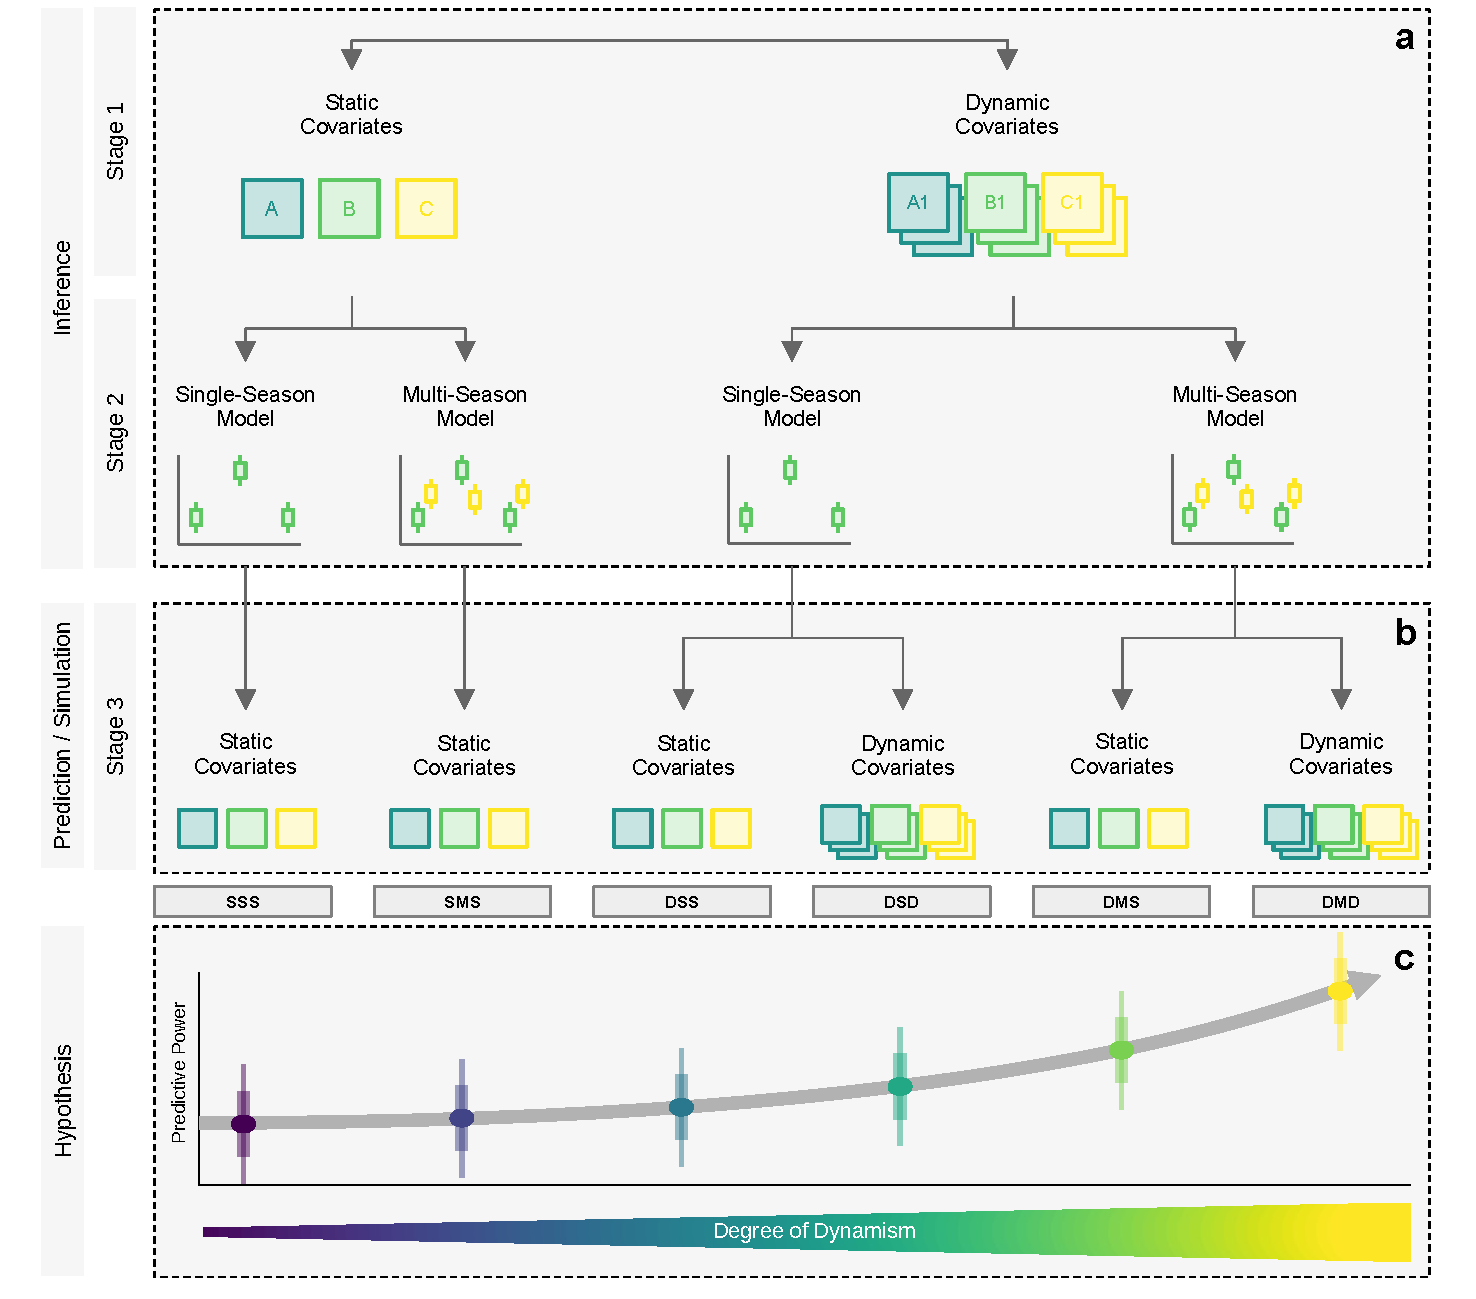
\includegraphics[width = \textwidth]{Figures/GraphicalAbstract.pdf}
  \caption{Overview of the different dimensions in which seasonality can be
  rendered in studies of landscape connectivity. (a) During model fitting, the
  modeler needs to decide whether to represent the environment by a static set
  of covariate layers, thus ignoring seasonality, or whether to obtain a dynamic
  set covariate layers that allow rendering it. One also needs to decide
  whether to parameterize a single-season model, assuming fixed preferences
  across the year, or to engage in a multi-season model that accounts for
  seasonal differences. (b) When utilizing the fitted model to predict
  connectivity, one can either assume a static set of environmental covariates
  or again attempt a seasonal take that renders how connectivity differs
  depending on the season. (c) Depending on these decisions, six different
  combinations with differing degrees of dynamism emerge. Our hypothesis was
  that increasing the degree of dynamism would lead to improved predictions.
  However, we were particularly interested in determining at which stage the
  inclusion of seasonally provided the biggest benefits.}
  \label{GraphicalAbstract}
 \end{center}
\end{figure}

\subsection{What We Did}

Here, we examined the importance of including seasonally-varying factors to
assess landscape connectivity for the African wild dog. For this, we compared
the predictive performance of iSSFs that differ in terms of the dynamism they
represented. Specifically, we investigate if and to what degree seasonality at
different stages of the connectivity modeling workflow contributes to improved
predictions. For this, we compile an extensive collection of remote sensed time
series data that accurately render seasonality across the Okavango Delta
ecosystem. We combine them with multi-year dispersal data from
\inputy{GeneralMetrics/CollarsTotal} dispersing wild dog coalitions in northern
Botswana and apply k-fold cross-validation for case-control studies to compare
the predictive efficacy of each model. Finally, we employ IBMMs to simulate
dispersal and estimate connectivity resulting from varying degrees of dynamism.
We hypothesized that habitat-selection and movement behavior would differ
significantly between seasons and that increasing the degree of dynamism would
result in better agreement between observed and predicted dispersal patterns
(\Cref{GraphicalAbstract}).

\section{Methods}

We used the \texttt{R} programming language \citep{RCoreTeam.2023} for all data
preparation and analyses. We performed spatial data manipulation using the
\texttt{terra} \citep{Hijmans.2024} and \texttt{spatstat} \citep{Baddeley.2015}
packages. We generated figures using the \texttt{ggplot2} \citep{Wickham.2024}
and \texttt{ggpubr} \citep{Kassambara.2024} packages. To ensure reproducibility
of all our analyses, we provide access to our \texttt{R}-scripts through an
online repository upon publication of this article.

\subsection{Study Area}

The study area comprised the Okavango Delta ecosystem, mainly within northern
Botswana (centered at \inputy{GeneralMetrics/StudyAreaCenter.tex} at an
elevation of approx. 950 m) but also extended to parts of Namibia and Zimbabwe,
and stretched across an extent of \inputy{GeneralMetrics/SizeStudyArea.tex}
km\textsuperscript{2} (\Cref{StudyArea}). The Okavango Delta is a flood-pulse
driven mosaic of patchy woodlands, permanent swamps, and seasonally flooded
grasslands that lie within the otherwise dry and sandy Kalahari Basin
\citep{Wilson.1976, Ramberg.2006, Mendelsohn.2010}. Precipitation across the
study area varies considerably between seasons, ranging from
\inputy{GeneralMetrics/MinimumPrecipitation.tex} mm during the dry season (from
$\sim$ 15 April to 15 October) to
\inputy{GeneralMetrics/MaximumPrecipitation.tex} mm during the wet season (from
$\sim$ 15 October to 15 April), totaling to
\inputy{GeneralMetrics/TotalPrecipitation.tex} mm across an average year
(\Cref{Seasonality}a). Daily maximum above-ground temperature fluctuates between
\inputy{GeneralMetrics/MinimumTemperature.tex}\degree C during the dry winter
months to \inputy{GeneralMetrics/MaximumTemperature.tex}\degree C during the wet
summer months (\Cref{Seasonality}b). The vegetation in the study area is mainly
composed of mopane forest (\textit{Colophospermum mopane}), mixed woodland
acacia-dominated (\textit{Acacia spp.}), and grassland. Substantial vegetation
green-up (e.g., plant and shoots growth, leaf production, grass greening) after
the dry season starts with a delay of some weeks after the onset of the first
rains in the wet season. The normalized difference vegetation index (NDVI)
therefore depicts a lagged response to precipitation patterns across the study
area (\Cref{Seasonality}c). The yearly flood-cycle of the Delta is predominantly
driven by rainfalls in the Angolan highlands, where water is collected and
channeled through the Cubango and Cuito rivers into the Okavango Delta
\citep{McCarthy.2003, Gumbricht.2004, Mendelsohn.2010}. Because water only
slowly descends from the catchment areas in Angola into the Delta's tributaries,
the flood is out of sync with local rainfalls and reaches its maximum extent
during August-September, i.e. during peak dry season (\citealp{Wolski.2017},
\Cref{Seasonality}d). While the extent of large-bodied rivers and floodplains is
determined by precipitation in Angola, the emergence of smaller, ephemeral
water-bodies (a.k.a., pans) is dictated by local precipitation during the wet
season. \inputy{GeneralMetrics/PercentageProtected.tex}\% of the landscape in
the study area form part of a protected area, such that human impact remains low
and largely limited to settlements along the western part of the delta and the
city of Maun at the delta's southern tip (\Cref{StudyArea}). Landscapes outside
protected areas in Zimbabwe, however, are more heavily influenced by humans,
mainly through agricultural fields and human settlements.

\begin{figure}
 \begin{center}
  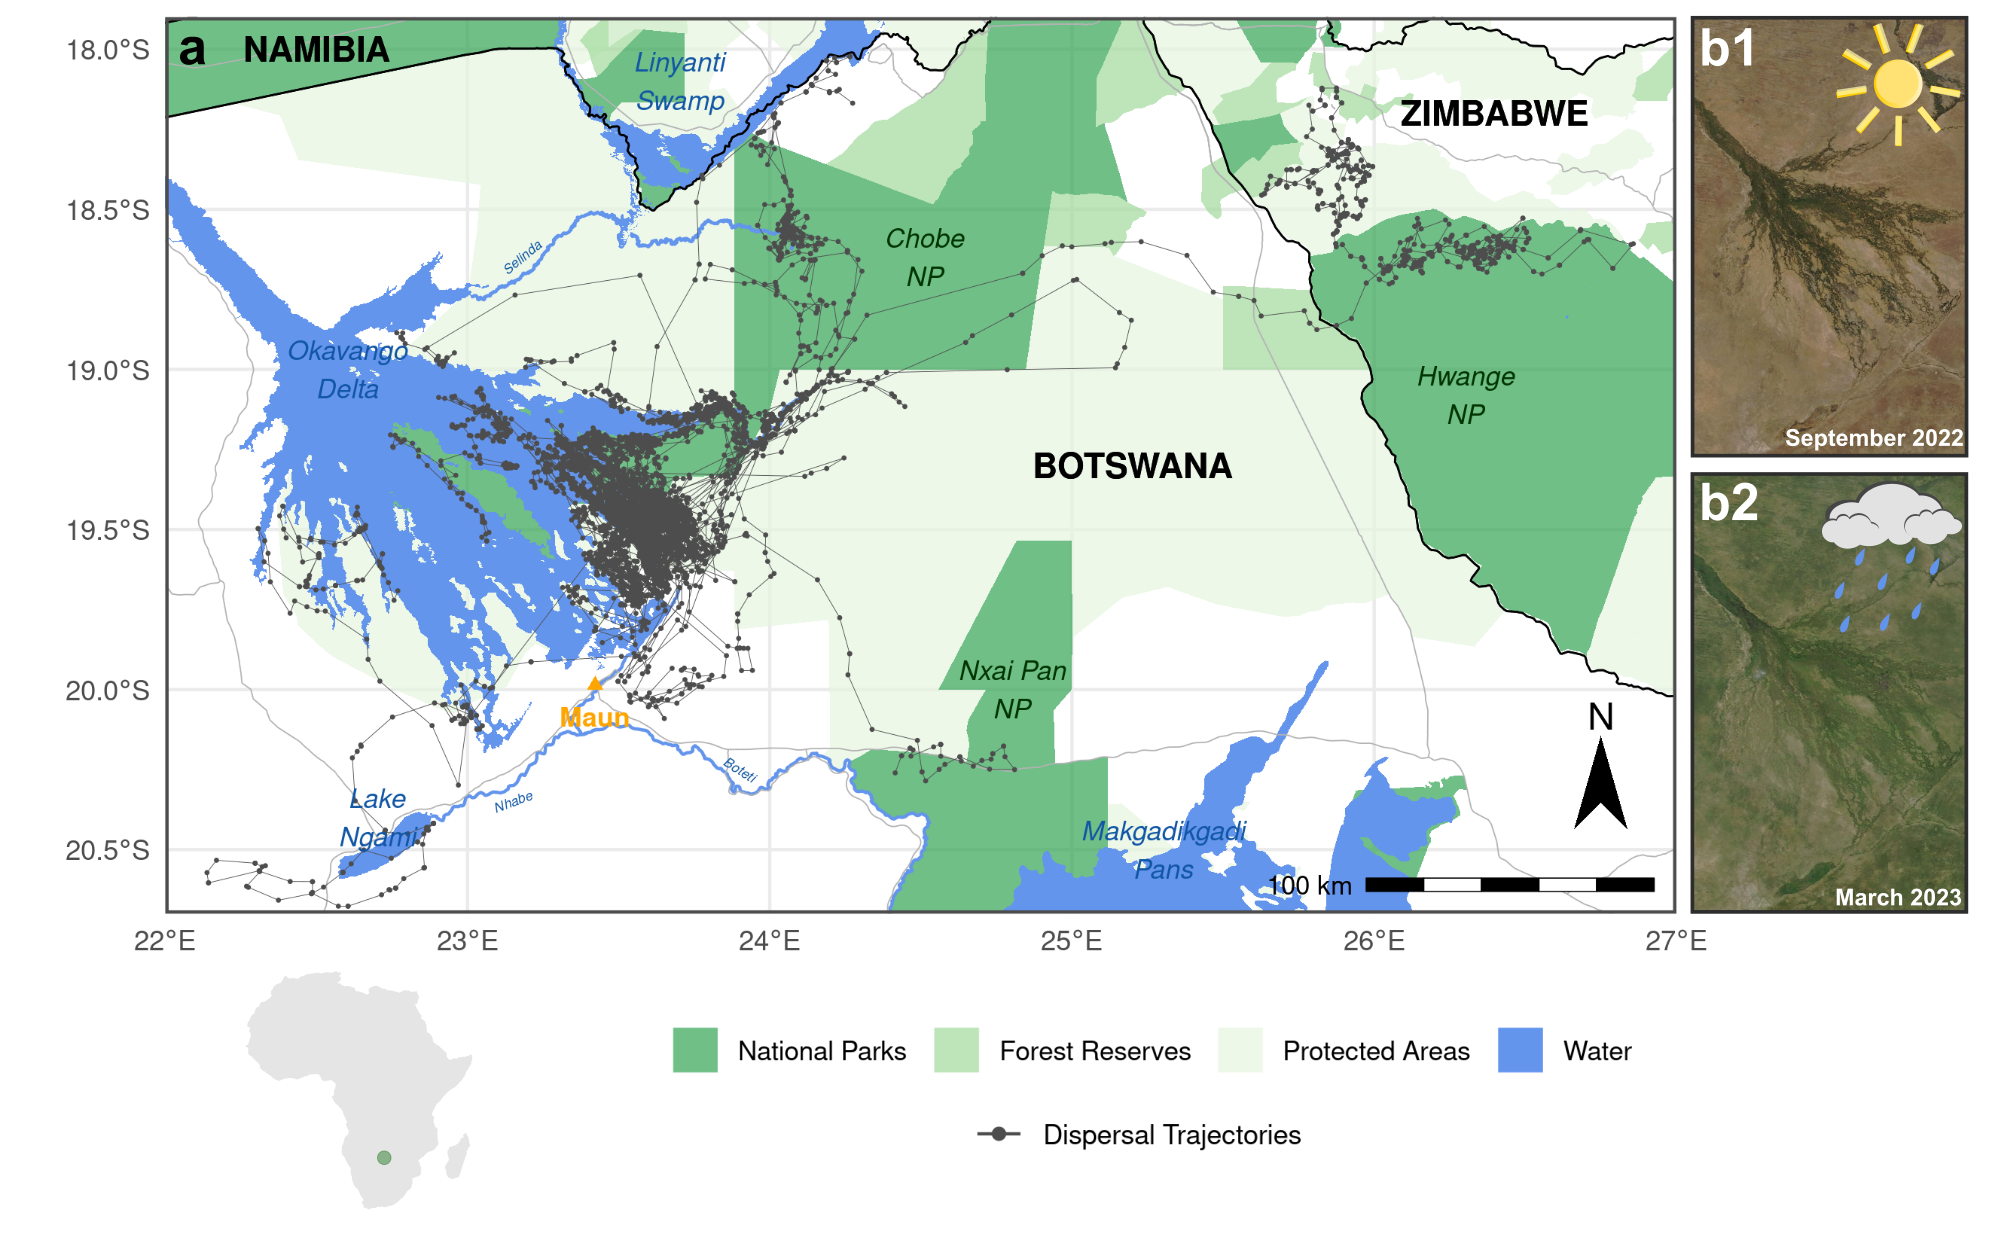
\includegraphics[width = \textwidth]{Figures/StudyArea.png} \caption{(a) Study
  area from which data on dispersing wild dogs were collected. Dispersal
  trajectories are plotted in dark gray. The study area encompassed parts of the
  Okavango Delta in northern Botswana, a highly dynamic, flood-pulse-driven
  ecosystem. The entire study area undergoes substantial seasonal changes, as
  can be seen from two satellite images taken during peak dry season (b1) and
  peak rainy season (b2). Notably, the flood of the Okavango Delta reaches its
  maximum extent during peak dry season (August–September).}
  \label{StudyArea}
 \end{center}
\end{figure}

\begin{figure}
\begin{center}
  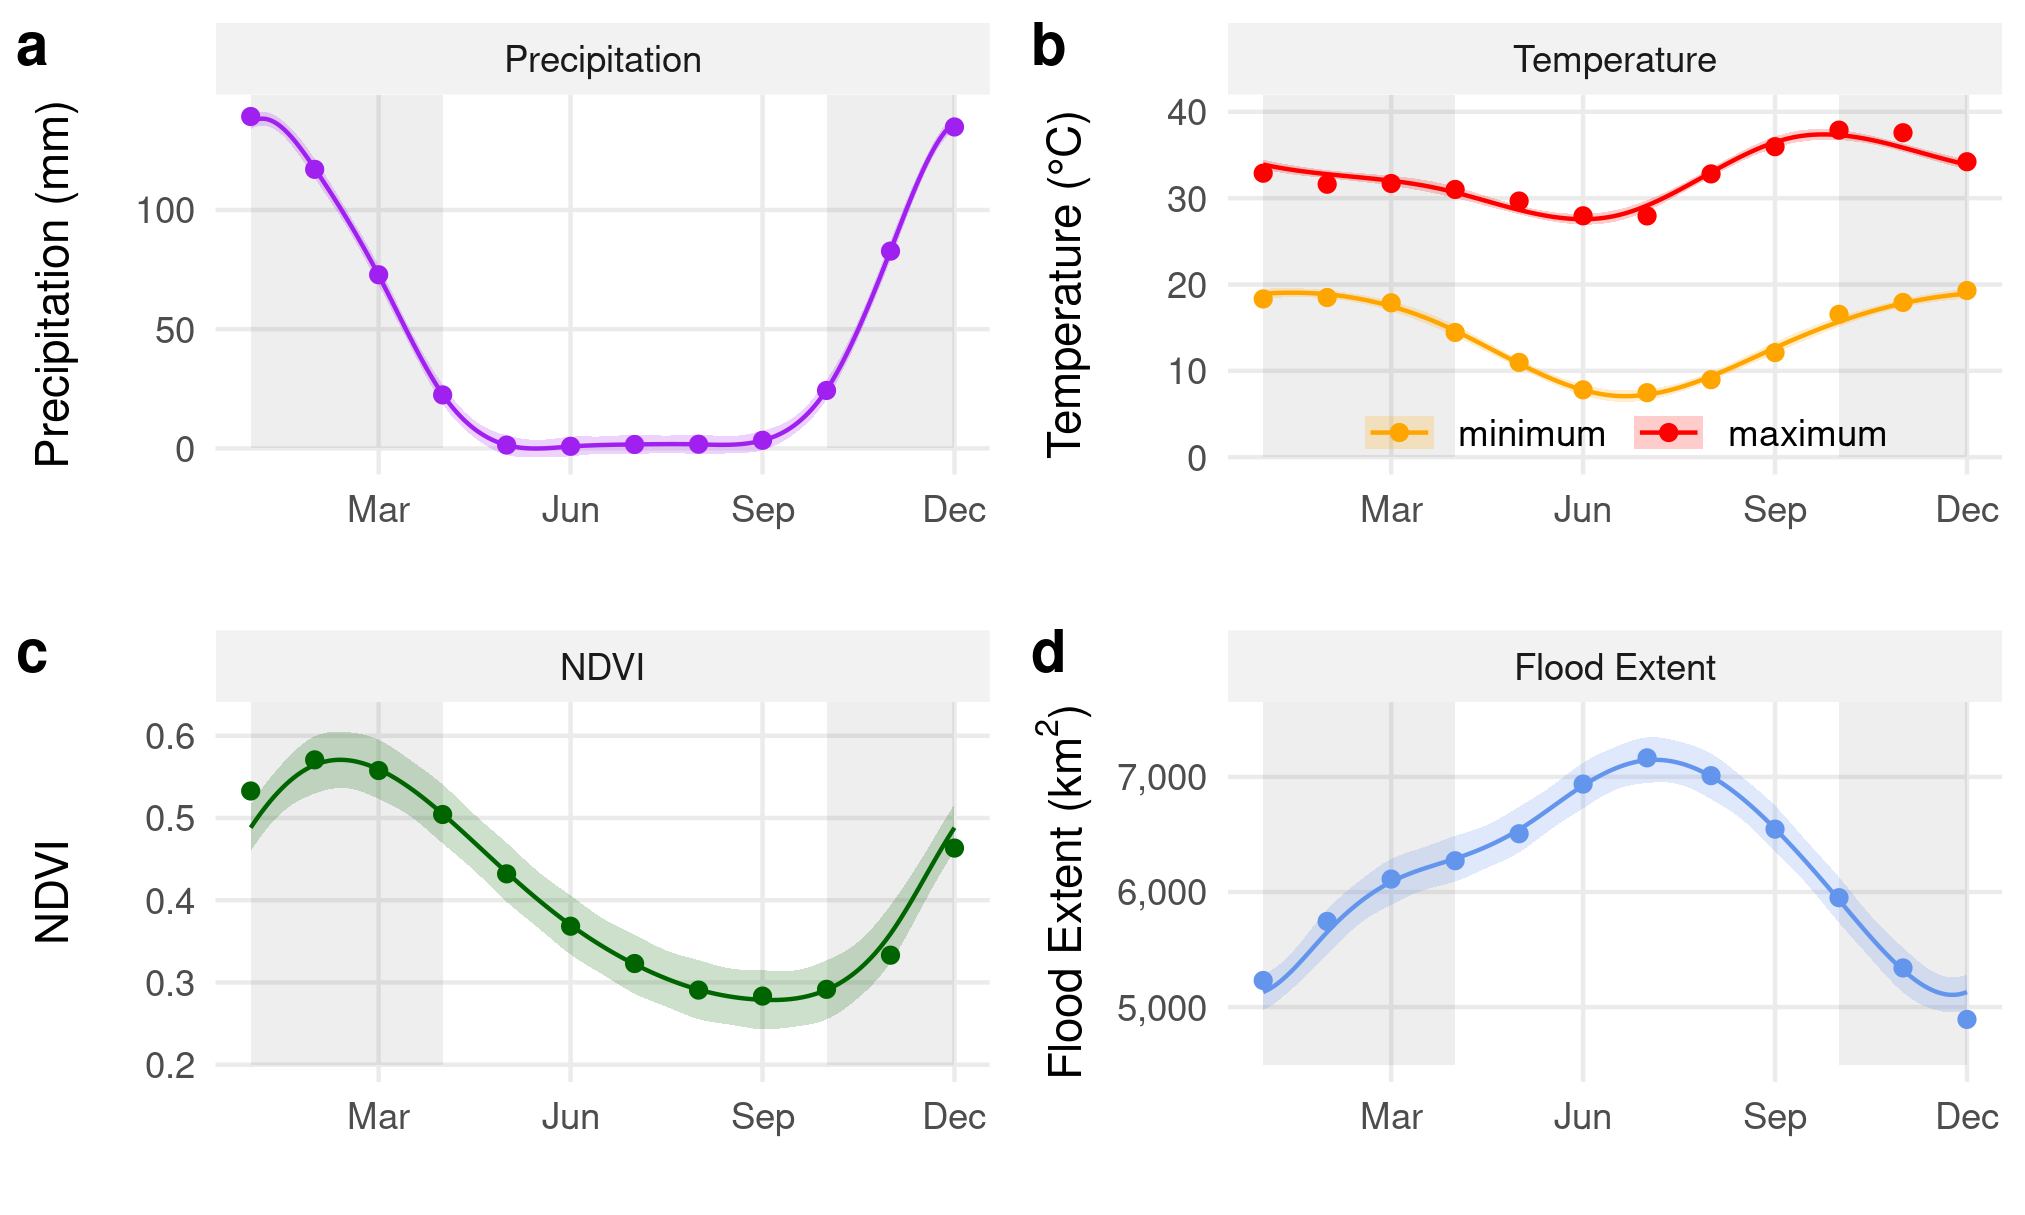
\includegraphics[width = \textwidth]{Figures/SeasonalCovariates.png}
  \caption{Illustration of how some covariates considered in this study vary
  across seasons. The wet season spans mid-October to mid-April (shaded in
  gray). Data for the graphs were obtained from \textbf{(a)} JAXA GSMaP,
  \textbf{(b)} ERA5, \textbf{(c)} MODIS MOD13Q1, and \textbf{(d)} remote sensed
  MOD43A4 satellite images. Smoothing curves were fitted using GAMs as
  implemented in the \texttt{mgcv} \texttt{R}-package \citep{Wood.2011}.}
  \label{Seasonality}
\end{center}
\end{figure}

\subsection{GPS Data}

Between \inputy{GeneralMetrics/GPSFromYear} and
\inputy{GeneralMetrics/GPSToYear}, we collected GPS data of
\inputy{GeneralMetrics/CollarsTotal} dispersing wild dog coalitions
(\inputy{GeneralMetrics/CollarsFemales} female coalitions,
\inputy{GeneralMetrics/CollarsMales} male coalitions \Cref{StudyArea}b). We
programmed GPS satellite collars to record GPS locations at 17:00, 21:00, 01:00,
05:00, and 09:00 o'clock. The eight-hour window between 09:00 and 17:00 can be
considered comparable to a four-hour window, as wild dogs generally rest between
11:00 and 15:00, leaving approximately four hours of activity
\citep{Hayward.2009}. The collected GPS data was regularly transmitted to a
base-station via Iridium satellite, thereby allowing dispersing individuals to
be monitored, even if they ventured across national borders. In total, we
obtained \inputy{GeneralMetrics/FixesTotal} locations during dispersal, with an
average of \inputy{GeneralMetrics/FixesMeanSD} locations per coalition.
Occasionally, the acquisition of a GPS location failed (success rate =
\inputy{GeneralMetrics/AcquisitionRate}\%), resulting in slight deviations from
the aspired four-hourly schedule. Further details on the GPS collar fitting
procedure and how we distinguished between dispersal and resident movements can
be found in \citet{Cozzi.2020} and \citet{Hofmann.2021}.

\subsection{Covariates}

We represented the physical landscape through which dispersers moved by a suite
of spatial covariate layers known to influence wild dog movements during
dispersal. We broadly categorized these spatial covariates into descriptors of
(1) landscape characteristics, (2) climatic conditions, and (3) anthropogenic
factors (\Cref{Covariates}) (see \citealp{Hofmann.2021, Hofmann.2023}). Besides
spatial covariates, we also prepared a series of covariates relating to (4)
light availability (\Cref{Covariates}) (see Cozzi et al. 2012). To appropriately
render seasonality in each of the spatial covariates (1-3), we downloaded them
at the highest spatial and temporal resolution available. That is, we obtained
for each spatial covariates by a stack of raster layers that spanned the entire
range of dates and locations for which we also collected GPS data of dispersing
wild dogs. Depending on the covariate, this resulted in differing spatial and
temporal resolutions (\Cref{Covariates}). Additionally, for each spatial
covariate, we also generated a static layer, representing ``average'' conditions
across the entire duration of the study. For this, we flattened each covariate
stack into a single layer, thus removing seasonality from the spatial data
entirely. For continuous covariates, we achieved this by averaging conditions
across all collected layers, whereas for categorical (binary) layers we
identified areas that were covered by the respective category in at least 50\%
of all layers. Using the same aggregation techniques, we computed covariate
stacks representative of a typical year. That is, instead of removing
seasonality by flattening across the entire range of dates, we flattened stacks
across years, thereby eliminating year-specific effects. These final layers
served to be used in the dispersal simulation, where we needed data representing
seasonality in all covariates across a typical year. To summarize, we prepared
each spatial covariate dynamically for the entire range of dates considered,
dynamically for an average year, and statically across the entire range of dates
considered.

\onehalfspacing
\begin{table}[htbp]
 \begin{center}
    \caption{Covariates that were used in this study, including information on
    their temporal and spatial resolutions, as well as on the avenue through which
    the respective data were accessed or downloaded.}
    \label{Covariates}
   \begin{threeparttable}
    \begin{tabular}{lcr}
      
\begin{tabular}[t]{lcccc}
\toprule
Variable & \makecell[c]{Temporal\\Resolution} & \makecell[c]{Spatial\\Resolution} & Source & \makecell[c]{Download\\Method}\\
\midrule
\addlinespace[0.3em]
\multicolumn{5}{l}{(1) Landscape Characteristics}\\
\hspace{1em}Trees & 1 year & 250 m & MODIS MOD44B & \texttt{RGISTools}\\
\hspace{1em}Shrubs / grassland & 1 year & 250 m & MODIS MOD44B & \texttt{RGISTools}\\
\hspace{1em}NDVI & 16 days & 250 m & MODIS MOD13Q1 & \texttt{rgee}\\
\cellcolor[HTML]{f2f2f2}{\hspace{1em}Rivers} & \cellcolor[HTML]{f2f2f2}{static} & \cellcolor[HTML]{f2f2f2}{90 m} & \cellcolor[HTML]{f2f2f2}{MERIT Hydro} & \cellcolor[HTML]{f2f2f2}{website}\\
\cellcolor[HTML]{f2f2f2}{\hspace{1em}Permanent water} & \cellcolor[HTML]{f2f2f2}{static} & \cellcolor[HTML]{f2f2f2}{30 m} & \cellcolor[HTML]{f2f2f2}{Globeland30} & \cellcolor[HTML]{f2f2f2}{website}\\
\cellcolor[HTML]{f2f2f2}{\hspace{1em}Floodwater} & \cellcolor[HTML]{f2f2f2}{8 days} & \cellcolor[HTML]{f2f2f2}{500 m} & \cellcolor[HTML]{f2f2f2}{MOD34A4} & \cellcolor[HTML]{f2f2f2}{\texttt{floodmapr}}\\
\hspace{1em}Distance to water & 8 days & 500 m & MOD43A4 & \texttt{floodmapr}\\
\hspace{1em}Pans & 5/10 days & 10 m & Sentinel 2 & \texttt{sen2r}\\
\hspace{1em}Distance to pans & 5/10 days & 10 m & Sentinel 2 & \texttt{sen2r}\\
\addlinespace[0.3em]
\multicolumn{5}{l}{(2) Climate Descriptors}\\
\hspace{1em}Temperature & 4 hours & 10 km & ERA5 & \texttt{rgee}\\
\hspace{1em}Precipitation & 4 hours & 10 km & JAXA GSMaP & \texttt{rgee}\\
\addlinespace[0.3em]
\multicolumn{5}{l}{(3) Anthropogenic Features}\\
\cellcolor[HTML]{f2f2f2}{\hspace{1em}Human density} & \cellcolor[HTML]{f2f2f2}{static} & \cellcolor[HTML]{f2f2f2}{30 m} & \cellcolor[HTML]{f2f2f2}{Facebook} & \cellcolor[HTML]{f2f2f2}{website}\\
\cellcolor[HTML]{f2f2f2}{\hspace{1em}Agriculture} & \cellcolor[HTML]{f2f2f2}{static} & \cellcolor[HTML]{f2f2f2}{30 m} & \cellcolor[HTML]{f2f2f2}{Globeland30 / Cropland} & \cellcolor[HTML]{f2f2f2}{website}\\
\cellcolor[HTML]{f2f2f2}{\hspace{1em}Roads} & \cellcolor[HTML]{f2f2f2}{static} & \cellcolor[HTML]{f2f2f2}{vectorized} & \cellcolor[HTML]{f2f2f2}{Open Street Map} & \cellcolor[HTML]{f2f2f2}{website}\\
\addlinespace[0.3em]
\multicolumn{5}{l}{(4) Light Availability}\\
\cellcolor[HTML]{f2f2f2}{\hspace{1em}Night} & \cellcolor[HTML]{f2f2f2}{4 hours} & \cellcolor[HTML]{f2f2f2}{-} & \cellcolor[HTML]{f2f2f2}{-} & \cellcolor[HTML]{f2f2f2}{\texttt{moonlit}}\\
\cellcolor[HTML]{f2f2f2}{\hspace{1em}Moon illumination} & \cellcolor[HTML]{f2f2f2}{4 hours} & \cellcolor[HTML]{f2f2f2}{-} & \cellcolor[HTML]{f2f2f2}{-} & \cellcolor[HTML]{f2f2f2}{\texttt{moonlit}}\\
\bottomrule
\end{tabular}

    \end{tabular}
    \begin{tablenotes}
      \item \textit{Note:} The covariates in gray were combined into proxies for
      water, human influence, and brightness, respectively. The detailed
      aggregation procedure is described by \citet{Hofmann.2021}.
    \end{tablenotes}
   \end{threeparttable}
 \end{center}
\end{table}
\doublespacing

\subsubsection{Landscape Characteristics}

We used data from the MODIS Vegetation Continuous Fields dataset (MOD44B V061;
\citealp{DiMiceli.2022}) to represent different vegetation types across the
study area. The MOD44B dataset comprises three continuous layers, depicting the
percentage cover of woodland, shrubs/grassland, and bareland, respectively. The
three layers added up to 100\%, so we dropped bareland from further analysis,
thus preventing perfect multi-collinearity. The MOD44B product is updated on day
65 of each year, so we used the \texttt{R}-package \texttt{RGISTools}
\citep{Perez-Goya.2020} to download yearly updated layers, each at a resolution
of 250m x 250m. We also obtained information on the normalized vegetation
difference index (NDVI) through the MODIS MOD13Q1 dataset \citep{Didan.2015},
which also has a resolution of 250m x 250m. This product is updated every 16
days, and we accessed the respective data through Google Earth Engine
\citep{Gorelick.2017} using the \texttt{R}-package \texttt{rgee}
\citep{Aybar.2024}. To depict large, permanent water-bodies, we employed the
Globeland30 dataset, from which we only retained the land-cover class water,
while setting all other categories to dryland. Similarly, we used the MERIT
Hydro dataset to obtain information on permanent rivers \citep{Yamazaki.2019}.
To dynamically render large water-bodies, particularly the floodwaters of the
Okavango Delta, we prepared weekly updated floodmaps using remote sensed MODIS
MOD43A4 satellite images. The underlying floodmapping algorithm is described in
detail in \citet{Wolski.2017} and \citet{Hofmann.2021} and is implemented in the
\texttt{floodmapr} package (available on GitHub;
\url{https://github.com/DavidDHofmann/floodmapr}). To generate a single layer
representing major water bodies, we combined the water, river, and flood layers
into a single stack with a resolution of 500m x 500m. Finally, we employed
remote sensing to detect small, ephemeral water bodies (i.e., pans) using a
custom random-forest classifier applied to Sentinel 2 satellite imagery
(\citealp{EuropeanSpaceAgency.2018}; details of the classifier in Appendix A1).
Sentinel 2 has a resolution of 10m and is therefore particularly useful for
obtaining information on small landscape features. Even though Sentinel 2
satellite imagery is updated every 5 days, cloud cover often prohibited the
computation of a ``pan-map''. Consequently, we settled for monthly updated
composite images, which effectively alleviated problems due to cloud cover. In
summary, we produced one stack of layers representing major water bodies, and
another stack of layers representing ephemeral water bodies. For both, we also
computed corresponding distance-to stacks.

\subsubsection{Climate Descriptors}

We obtained hourly updated spatial layers on 2m above-ground temperature from
the ERA5-Land dataset \citep{Munoz-Sabater.2021} and hourly updated
precipitation estimates from the Global Satellite Mapping of Precipitation
dataset \citep{Kubota.2020}. Both datasets were accessed and downloaded through
Google Earth Engine \citep{Gorelick.2017} using the \texttt{rgee} package
\citep{Aybar.2024} and had a resolution of 10km x 10km. To match hourly
temperature and precipitation values with the four-hourly data collected by the
GPS satellite collars fitted on the dispersing wild dogs, we computed average
precipitation and temperature values over four hourly periods that matched the
GPS collection schedule.

\subsubsection{Anthropogenic Features}

We combined information on human density, agricultural activities, and roads
into a single proxy, which we generically termed human influence. We sourced
information on human density from Facebook's high resolution human density
dataset \citep{Tiecke.2017}, which we downloaded from the humdata website
(\url{www.data.humdata.org/}). We obtained information on the presence of
agricultural fields from the Globeland30 \citep{Chen.2015} and Cropland
\citep{Xiong.2017} datasets. We  downloaded shapefiles comprising main tar roads
from OpenStreetMaps \citep{OpenStreetMapContributors.2017}. Ultimately, we
merged all anthropogenic features into a single layer (details in
\citealp{Hofmann.2021}) that had a resolution of 250m x 250m.

\subsubsection{Light Availability}

We computed light statistics using the \texttt{suncalc} and \texttt{moonlit}
\texttt{R}-packages \citep{Thieurmel.2022, Smielak.2023} for the central
coordinates of our study area at a 5-minute temporal resolution. The set of
light statistics comprised a binary variable separating day and night (i.e., sun
$<$ -18 \degree below the horizon) and a continuous estimate of moonlight
illumination (relative to the maximum moon illumination). Based on those
covariates, we generated a binary covariate separating bright from dark
conditions. To provide a general understanding of this variable, bright
conditions encompassed all daytime hours and those nighttime periods during
which the moon was present in the sky and illuminated by approximately
one-fourth; conversely, dark conditions included nighttime periods during which
the moon was absent from the sky or present or was only minimally illuminated
(further details in Appendices A2 and A3).

\subsection{Step-Selection Models}

We modeled habitat selection and movement behavior of dispersing wild dogs using
integrated step-selection functions (iSSFs, \citealp{Fortin.2005, Avgar.2016}),
following the procedure described in \citet{Muff.2020}. For this, we identified
bursts of subsequent GPS locations where the duration between two GPS locations
did not exceed 4 hours (\(\pm\) 15 minutes) or 8 hours (\(\pm\) 30 minutes, for
data recorded between 09:00 and 17:00). Within each burst, we converted
locations into steps, where a step represented the straight line segment between
two consecutive locations \citep{Turchin.1998}. For each step, we computed the
associated step length (sl, in meters) and relative turning angle (ta, in
radians). After this pre-processing, a total of \inputy{GeneralMetrics/SSFTotal}
dispersing coalitions (\inputy{GeneralMetrics/SSFFemales} female coalitions,
\inputy{GeneralMetrics/SSFMales} male coalitions) remained for further analyses.
The final dataset comprised \inputy{GeneralMetrics/StepsTotal} steps
(\inputy{GeneralMetrics/StepsMeanSD} per coalition), which we further
categorized into wet (15 October to 15 April) and dry (15 April to 15 October)
season, resulting in \inputy{GeneralMetrics/NumberStepsDry} steps
(\inputy{GeneralMetrics/PercentageStepsDry}\%) during the dry season and
\inputy{GeneralMetrics/NumberStepsWet} steps
(\inputy{GeneralMetrics/PercentageStepsWet}\%) during the wet season.

We paired each \textit{observed} step with a set of 100 \textit{random} steps,
generated by sampling turning angles from  a uniform distribution U(\(-\pi,
+\pi\)) and step lengths from a gamma distribution fitted to observed steps
(scale \(\theta\) = \inputy{GeneralMetrics/GammaScale} and shape \(k\) =
\inputy{GeneralMetrics/GammaShape}). Together, an observed step and its
associated random steps formed a stratum that received a unique identifier.
Along each step, we extracted covariate values from the underlying spatial
habitat layers, and we assigned the appropriate light conditions
(\Cref{Covariates}). We opted for covariate extraction \textit{along} steps
rather than \textit{at their endpoints}, as we believed that environmental
conditions along steps were relevant in determining wild dog movement. For
continuous covariates, we computed average values along each step, for
categorical covariates the percentage cover of each category along the step. To
model a decreasing marginal impact of ``distance to'' variables, we included
their square-root as predictors in the final models. To facilitate model
convergence, we normalized extracted values to a range between 0 and 1.

To estimate habitat and movement parameters of interest, we applied the maximum
likelihood procedure proposed by \citet{Muff.2020}, using the \texttt{glmmTMB}
package \citep{Brooks.2017}. Our model formula was based on knowledge from
previous studies on dispersing wild dogs \citep{Hofmann.2021, Hofmann.2023} and
comprised a movement kernel (describing movement preferences), a
habitat-selection function (describing habitat preferences) and their
interactions (describing how movement differs depending on habitat conditions).
Notably, we included descriptors of the step length and turning angle (sl,
log(sl), and cos(ta)) in the regression model \citep{Avgar.2017, Fieberg.2021}.
We also fitted a stratum-specific intercept with a large fixed variance ($10^6$,
\citealp{Muff.2020}), and used dispersing coalition ID to model random slopes.
To examine whether the effect of accounting seasonality differed depending on
the employed model, we fit models either \textit{excluding} interactions
(hereafter called simple model) or \textit{including} interactions (hereafter
called full model). Specifically, in the simple model we only included
covariates relating to landscape characteristics and anthropogenic features in
the simple model, as well as the step-descriptors mandatory for conducting an
iSSF (i.e., sl, log(sl), and cos(ta); \citealp{Avgar.2016}). In the full model,
however, we included additional interactions with climatic descriptors and light
conditions, rendering that wild dog dispersal behavior may vary depending on
those. As such, the structure of the simple model can be viewed as a model
structure that is usually employed in permeability-based studies, which are
restricted to spatial covariates. The model structure of the full model,
conversely, included additional complexities that can only be accounted for when
investigating connectivity vis IBMMs. To ensure comparability among each of the
six configurations presented in our framework, we employed the same models
across all of them. Specifically, we fitted models that differed in their degree
of dynamism (\Cref{GraphicalAbstract}a). Models one and two were fit using
static covariates (\Cref{GraphicalAbstract}a, Stage 1), with model one being a
single-season model and model two being a multi-season model (wet vs. dry,
\Cref{GraphicalAbstract}a, Stage 2). Models two and three, by contrast, were fit
using dynamic covariates, with model three being a single-season model, and
model four being a multi-season model (wet vs. dry, \Cref{GraphicalAbstract}a,
Stage 2). To quantify how many random steps were necessary before model
estimates stabilized (sensu \citealp{Fieberg.2021}), we fitted each model with
5, 10, 25, 50, 75, and 100 random steps.

\subsection{Validation}

We compared the predictive efficacy of each of the six configurations
(\Cref{GraphicalAbstract}b) using k-fold cross-validation for case-control
studies \citep{Fortin.2009}. For this, we split the data into training and
validation sets using an 80:20 ratio and fitted the four iSSF models described
above. We then used the $\beta$-estimates to predict the probability of each
random and observed step in the validation set for being chosen. Depending on
the configuration, we predicted step-probabilities using static or dynamic
covariates. Within each stratum, we assigned ranks 1-101 to each step based on
predicted probabilities and recorded the number of times the observed step was
assigned each rank. Finally, we computed Spearman's rank correlation between
ranks and associated frequencies $r_{s, realized}$. The better a model's
predictive ability, the more negative $r_{s, realized}$ should be (i.e., the
less often the observed step should be assigned a low rank). For reference, we
also computed Spearman's rank correlation for randomized preferences ($r_{s,
random}$), which we achieved by removing the observed step from each stratum and
identifying the rank of a randomly chosen step. We replicated this validation
procedure 100 times and computed the mean correlation coefficient $\bar{r}_{s,
realized}$ and $\bar{r}_{random}$, as well as their 95\% percentiles across
replicates. Ultimately, this validation proves a significant prediction in case
the confidence intervals of \(\bar{r}_{s, realized}\) and \(\bar{r}_{s,
random}\) do not overlap \citep{Fortin.2009}.

\subsection{Simulations}

To assess differences in connectivity upon increasing seasonal dynamism, we ran
dispersal simulations under the two most distinct configurations, i.e. the fully
static (SSS, \Cref{GraphicalAbstract}) and fully dynamic (DMD,
\Cref{GraphicalAbstract}) configurations. As source areas to initiate
dispersers, we defined three distinct regions known to host viable wild dog
populations (\Cref{StudyArea}). The definition of these areas was somewhat
arbitrary, albeit we deliberately selected areas in the west and east of the
Delta to examine potential influences of flooding on connectivity
\citep{Hofmann.2024}, as well as a more isolated location that was not
influenced directly by the Delta's flood extent. To initiate simulated dispersal
trajectories, we randomly placed 1,000 start points within each of these source
area, with start times that were equally distributed across the year. To
simulate dispersal and obtain connectivity maps under both configurations, we
applied the simulation algorithm for iSSFs described in \citet{Signer.2017} and
employed in \citet{Hofmann.2023}. A similar algorithm has recently been added to
the \texttt{amt} \texttt{R}-package \citep{Signer.2024}. We applied the
simulation algorithm as follows. Originating from the start point, we generated
a set of 25 random steps by sampling step lengths from the fitted gamma
distribution and turning angles from a uniform distribution. Along each random
step, we extracted spatial covariates, computed relevant movement metrics (sl,
log(sl), and cos(ta)), and assigned light conditions. We then employed the
fitted iSSF model to predict the probability of each step for being chosen (i.e.
the redistribution kernel). Based on assigned probabilities, we sampled one of
the steps and updated the simulated individual's position and time. We repeated
the procedure until a total of 2,000 steps were realized ($\sim$ 400 dispersal
days).

Depending on the configuration, we employed different spatial covariates during
the simulation. For the SMS configuration, we used the static set of covariates,
which omitted any seasonality and assumed a static landscape over time. For the
DMD configuration, on the other hand, we updated covariates dynamically as the
simulated individuals moved. More specifically, we generated a new covariate
stack after every simulated step, comprising spatial layers that best
represented environmental conditions at that particular point in time
(\Cref{Schematic}). Note that we used the set of covariates representing an
average year for this purpose. For both configurations, we ultimately obtained a
heatmap (or utilization distribution) based on simulated trajectories. We also
generated difference maps between the two configurations, highlighting areas
where the difference in simulated connectivity were most pronounced.

\begin{figure}
 \begin{center}
  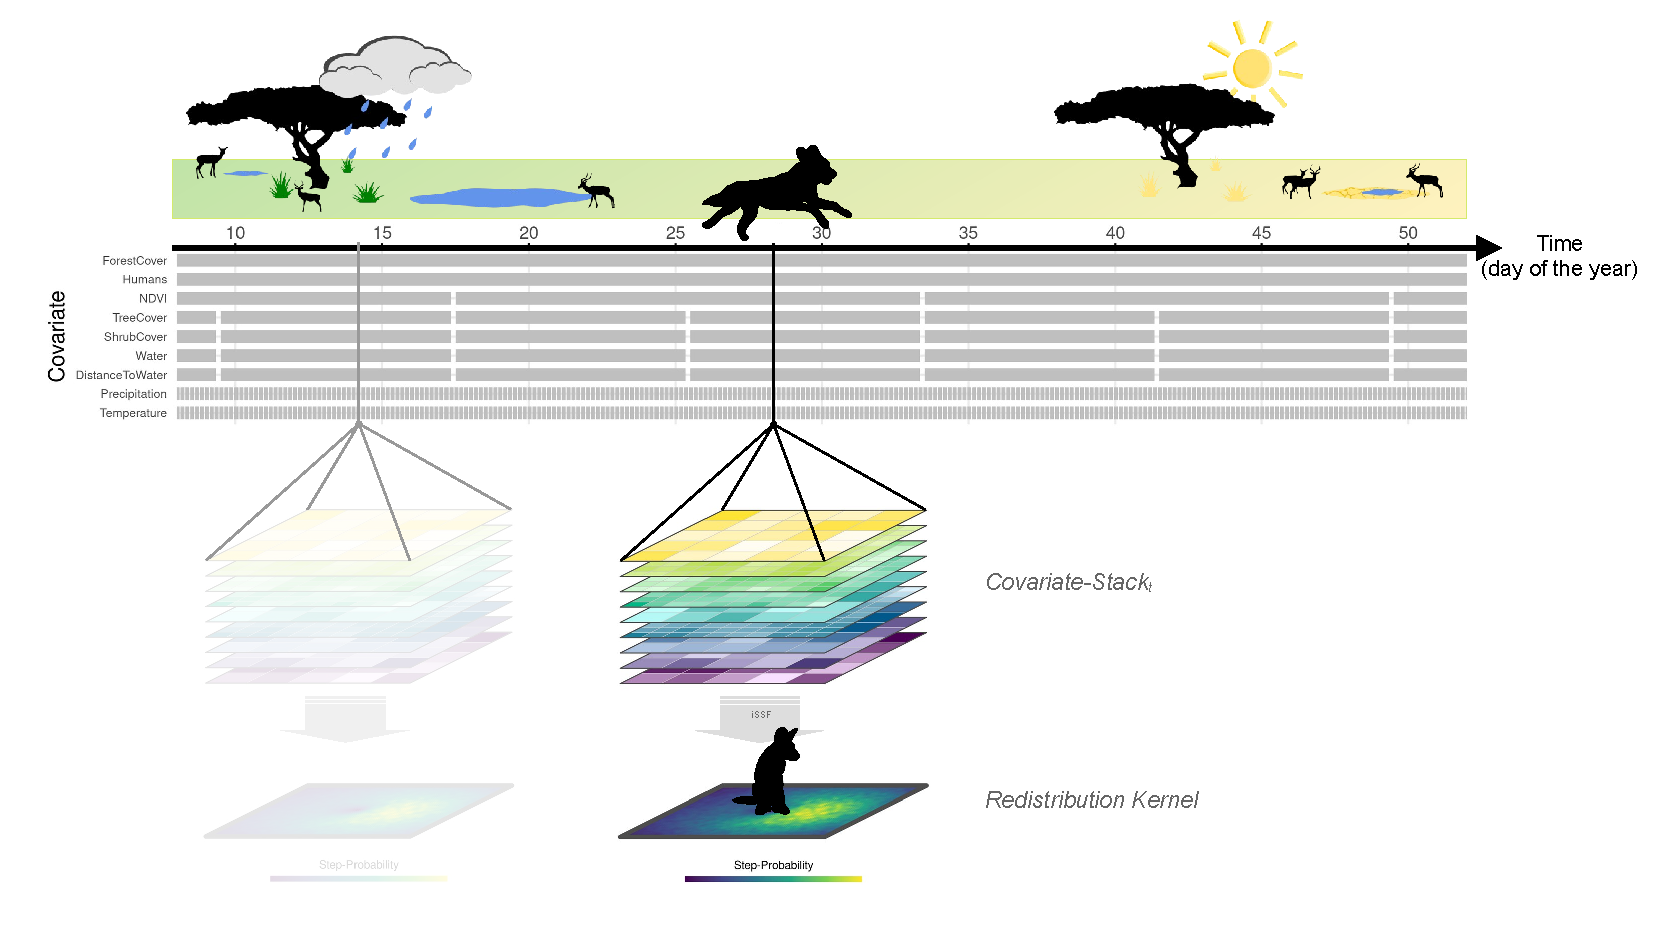
\includegraphics[width = \textwidth]{Figures/Schematic} \caption{Schematic
  illustration of a dispersal simulation with dynamic covariates. As the
  simulation proceeds, the underlying covariates (symbolized by the stack of
  layers) are updated. In our case, the update frequency of covariate layers
  varied from a few hours (e.g., temperature) to multiple months (e.g., shrub
  cover). Each gray block represents a single layer and the duration for which
  it was ``active''. Originating from the current position of the simulated
  animal, a new redistribution kernel is derived. We generated redistribution
  kernels by proposing a set of random steps and applying the parametrized
  step-selection model to predict the probability of each step for being chosen.
  Based on this kernel, one location was randomly sampled and the animal's
  position updated. This procedure was repeated until the number of simulated
  steps matched the number of steps from the observed individuals.}
  \label{Schematic}
 \end{center}
\end{figure}

\section{Results}

Due to convergence issues, we removed the covariates NDVI, precipitation, and
distance to pans from all analyses. Some minor convergence issues remained and
our validation procedure failed in 59 out of 1,800 validation attempts. Since
failures occurred across different configurations and were not clustered around
one specific configuration, we deemed their exclusion of no concern.

\subsection{Step-Selection Models}

Patterns of habitat selection and movement behavior were qualitatively similar,
irrespective of whether models were fit using static or dynamic covariates
(\Cref{MovementModel}, Tables S3, S4, S5, S6) and irrespective of the number of
considered random steps (Figure S9). The most notable quantitative difference
when using static vs. dynamic covariates (see \Cref{GraphicalAbstract}a) was
that models fitted using dynamic covariates resulted in narrower confidence
intervals (\Cref{MovementModel}). Furthermore, effect sizes (i.e.,
$\beta$-estimates) of models fit using static covariates were more pronounced
than effect sizes from models that were fit using dynamic covariates
(\Cref{MovementModel}). Differences were most marked for
$\beta_{DistanceToWater^{0.5}}$, which was estimated $\approx -0.8$ using static
covariates, but $\approx -0.3$ when using dynamic covariates.

Differences in $\beta$-estimates between seasons were moderate and most
pronounced when models were fit using static covariates. For instance, when
models were fit using static covariates, $\beta_{Water}$ was $\approx -1.1$
during the dry season but ($\approx 0.2$ during the wet season). When dynamic
covariates were used, by contrast, $\beta_{Water}$ was ($\approx -0.6$ and
$\approx -0.3$), respectively. $\beta_{sl:Dark}$ was also markedly lower during
the wet season ($\approx -0.9$), compared to the dry season ($\approx -0.1$).
Plots that aid with the interpretation of the resulting models are provided in
Figure S10.

\begin{figure}
 \begin{center}
  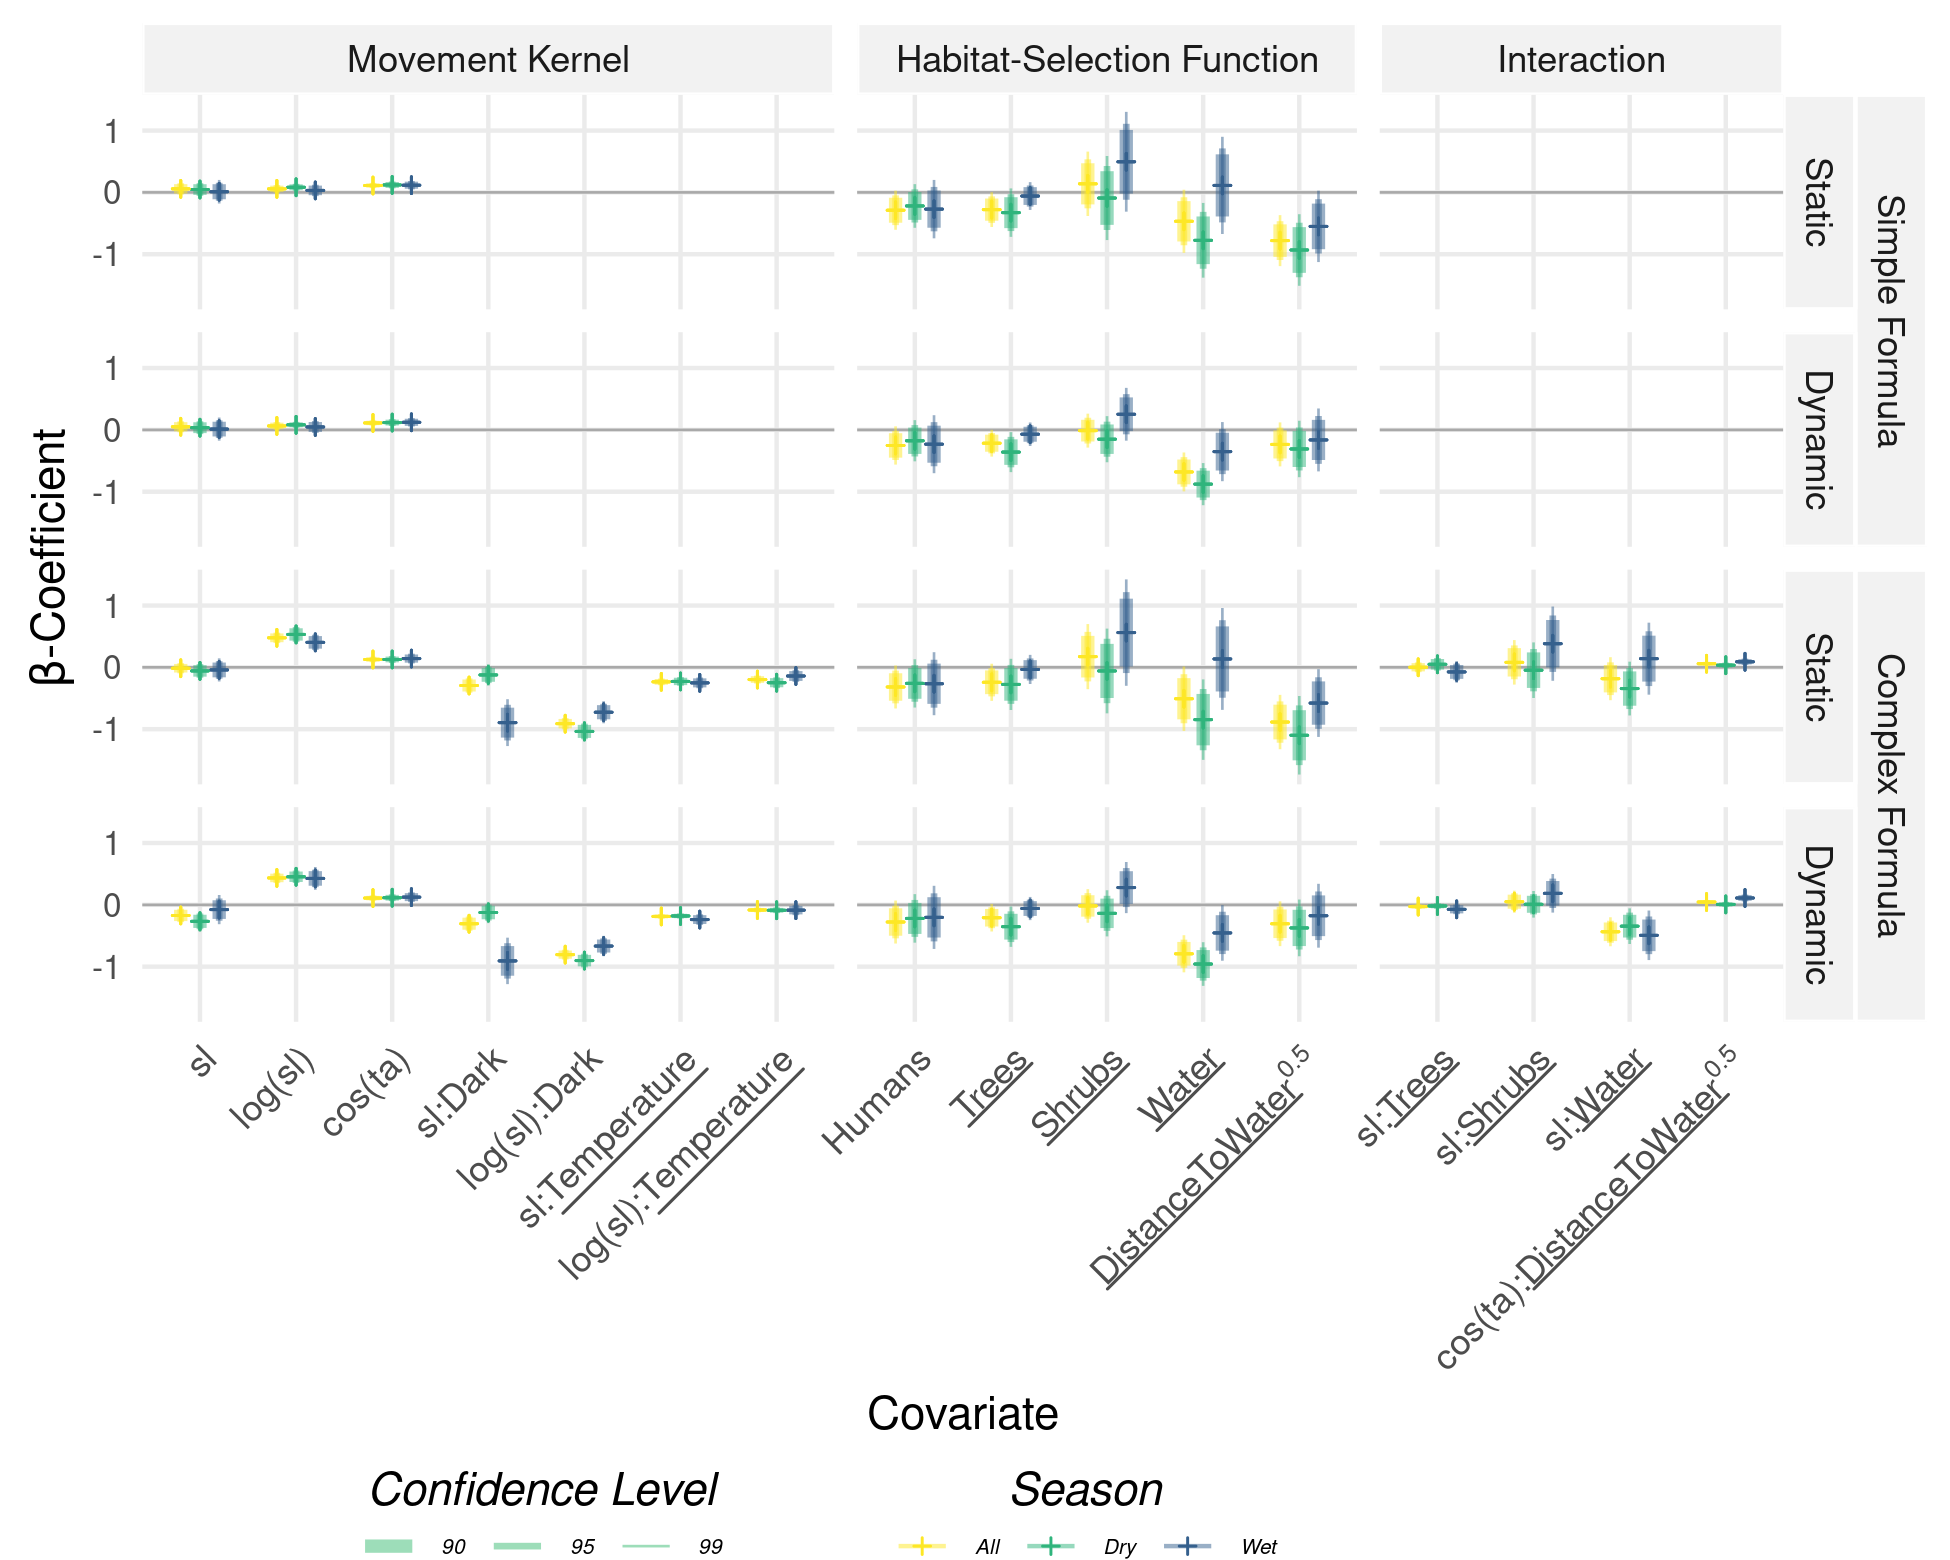
\includegraphics[width = \textwidth]{Figures/MovementModel.png}
  \caption{$\beta-$estimates from the integrated step-selection models, grouped
  by movement kernel, habitat-selection function, and their interaction. We
  either fit a simple model without interactions or a full model with
  interactions and we distinguished between models fit using static or dynamic
  covariates. Only the underlined covariates differed between the static and
  dynamic configurations, as covariates were either represented as a single
  layer (static), or a stack of layers (dynamic). Furthermore, data was either
  pooled across seasons (yellow bars) or split into dry (green bars) and wet
  (blue bars) season.}
  \label{MovementModel}
 \end{center}
\end{figure}

\subsection{Validation}

Spearman's rank correlation coefficients ($r$) obtained from the validation
procedure revealed that predictions from the full model performed better than
those from the simple model ($\bar{r}_{simple} = -0.5$, $\bar{r}_{full} = -0.9$,
\Cref{RankCorrelation}). Irrespective of the employed model, Spearman's rank
correlation differed significantly depending on the amount of dynamism
considered (simple: F(5, 593) = 26.45, p < 0.001, full: F(5, 594) = 7.14, p <
0.001), albeit with moderate effect sizes. In the simple model, moving from a
fully static (SSS) to a fully dynamic (DMD) configuration decreased Spearmans's
rank correlation (i.e., increased the predictive performance) by 0.15 from -0.41
to -0.56. In the full model, moving from a fully static (SSS) to a fully dynamic
(DMD) configuration entailed an increase in $r$ (i.e. a decrease in the
predictive performance) from -0.89 to -0.88. This suggests that, our hypothesis
that increased dynamism results in better predictive performance only holds with
the simple model (\Cref{RankCorrelation}a), but not the full model
(\Cref{RankCorrelation}b).

\begin{figure}
 \begin{center}
  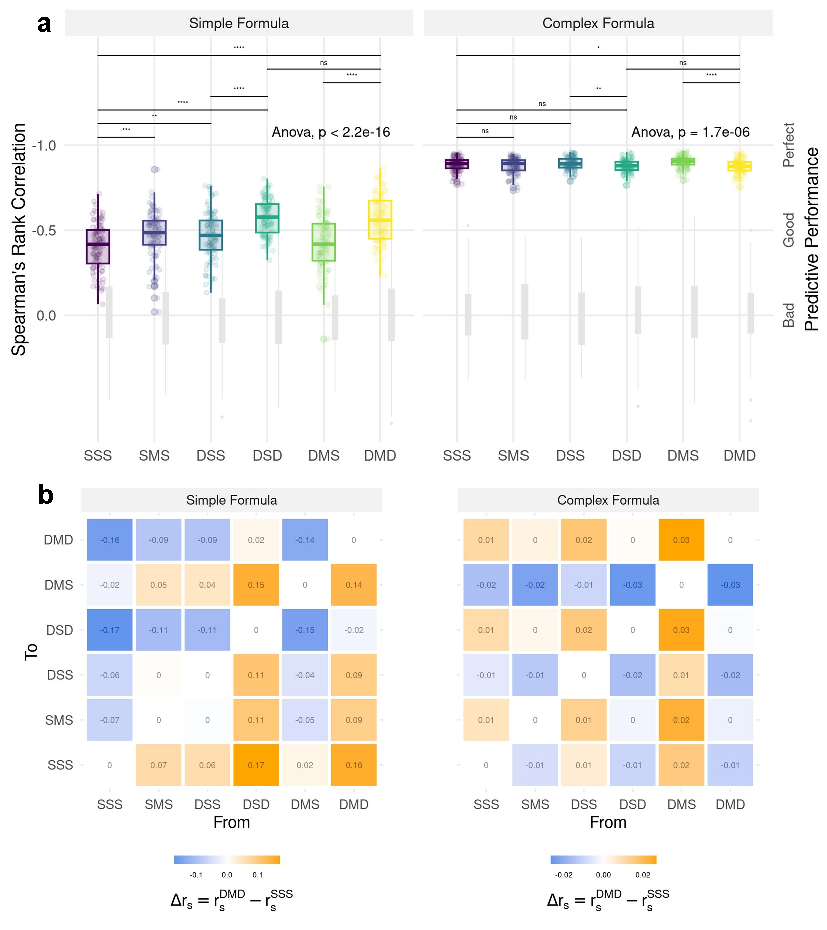
\includegraphics[width = \textwidth]{Figures/RankCorrelation.pdf}
  \caption{(a) Spearman's rank correlation across different configurations of
  dynamism that range from entirely static (SSS) to fully dynamic (DMD). The
  more negative Spearman's rank correlation, the better is the predictive
  performance under the respective configuration. Correlations were computed for
  100 replicates. Note that the y-axis is inverted to match our expectation of
  increasing performance as dynamism increases. (b) Difference in Spearman's
  rank correlation when moving from one configuration to another. Values $< 0$
  (blue) indicate an increase in predictive performance, whereas values $> 0$
  (orange) indicate a decrease in predictive performance.}
  \label{RankCorrelation}
 \end{center}
\end{figure}

\subsection{Simulations}

Simulations under the most static (SSS) and dynamic (DMD) configurations
revealed different connectivity patterns (\Cref{HeatmapComparison}). In the
static configuration, simulated dispersal trajectories more concentrated,
resulting in frequent movement across a few key habitats. In the dynamic
configuration, by contrast, simulated trajectories were more homogeneously
distributed. Qualitatively, connectivity patterns appeared similar between the
simple and full models. Given the similarities in habitat selection emerging
under the two models, this was to be expected.

\begin{figure}
 \begin{center}
  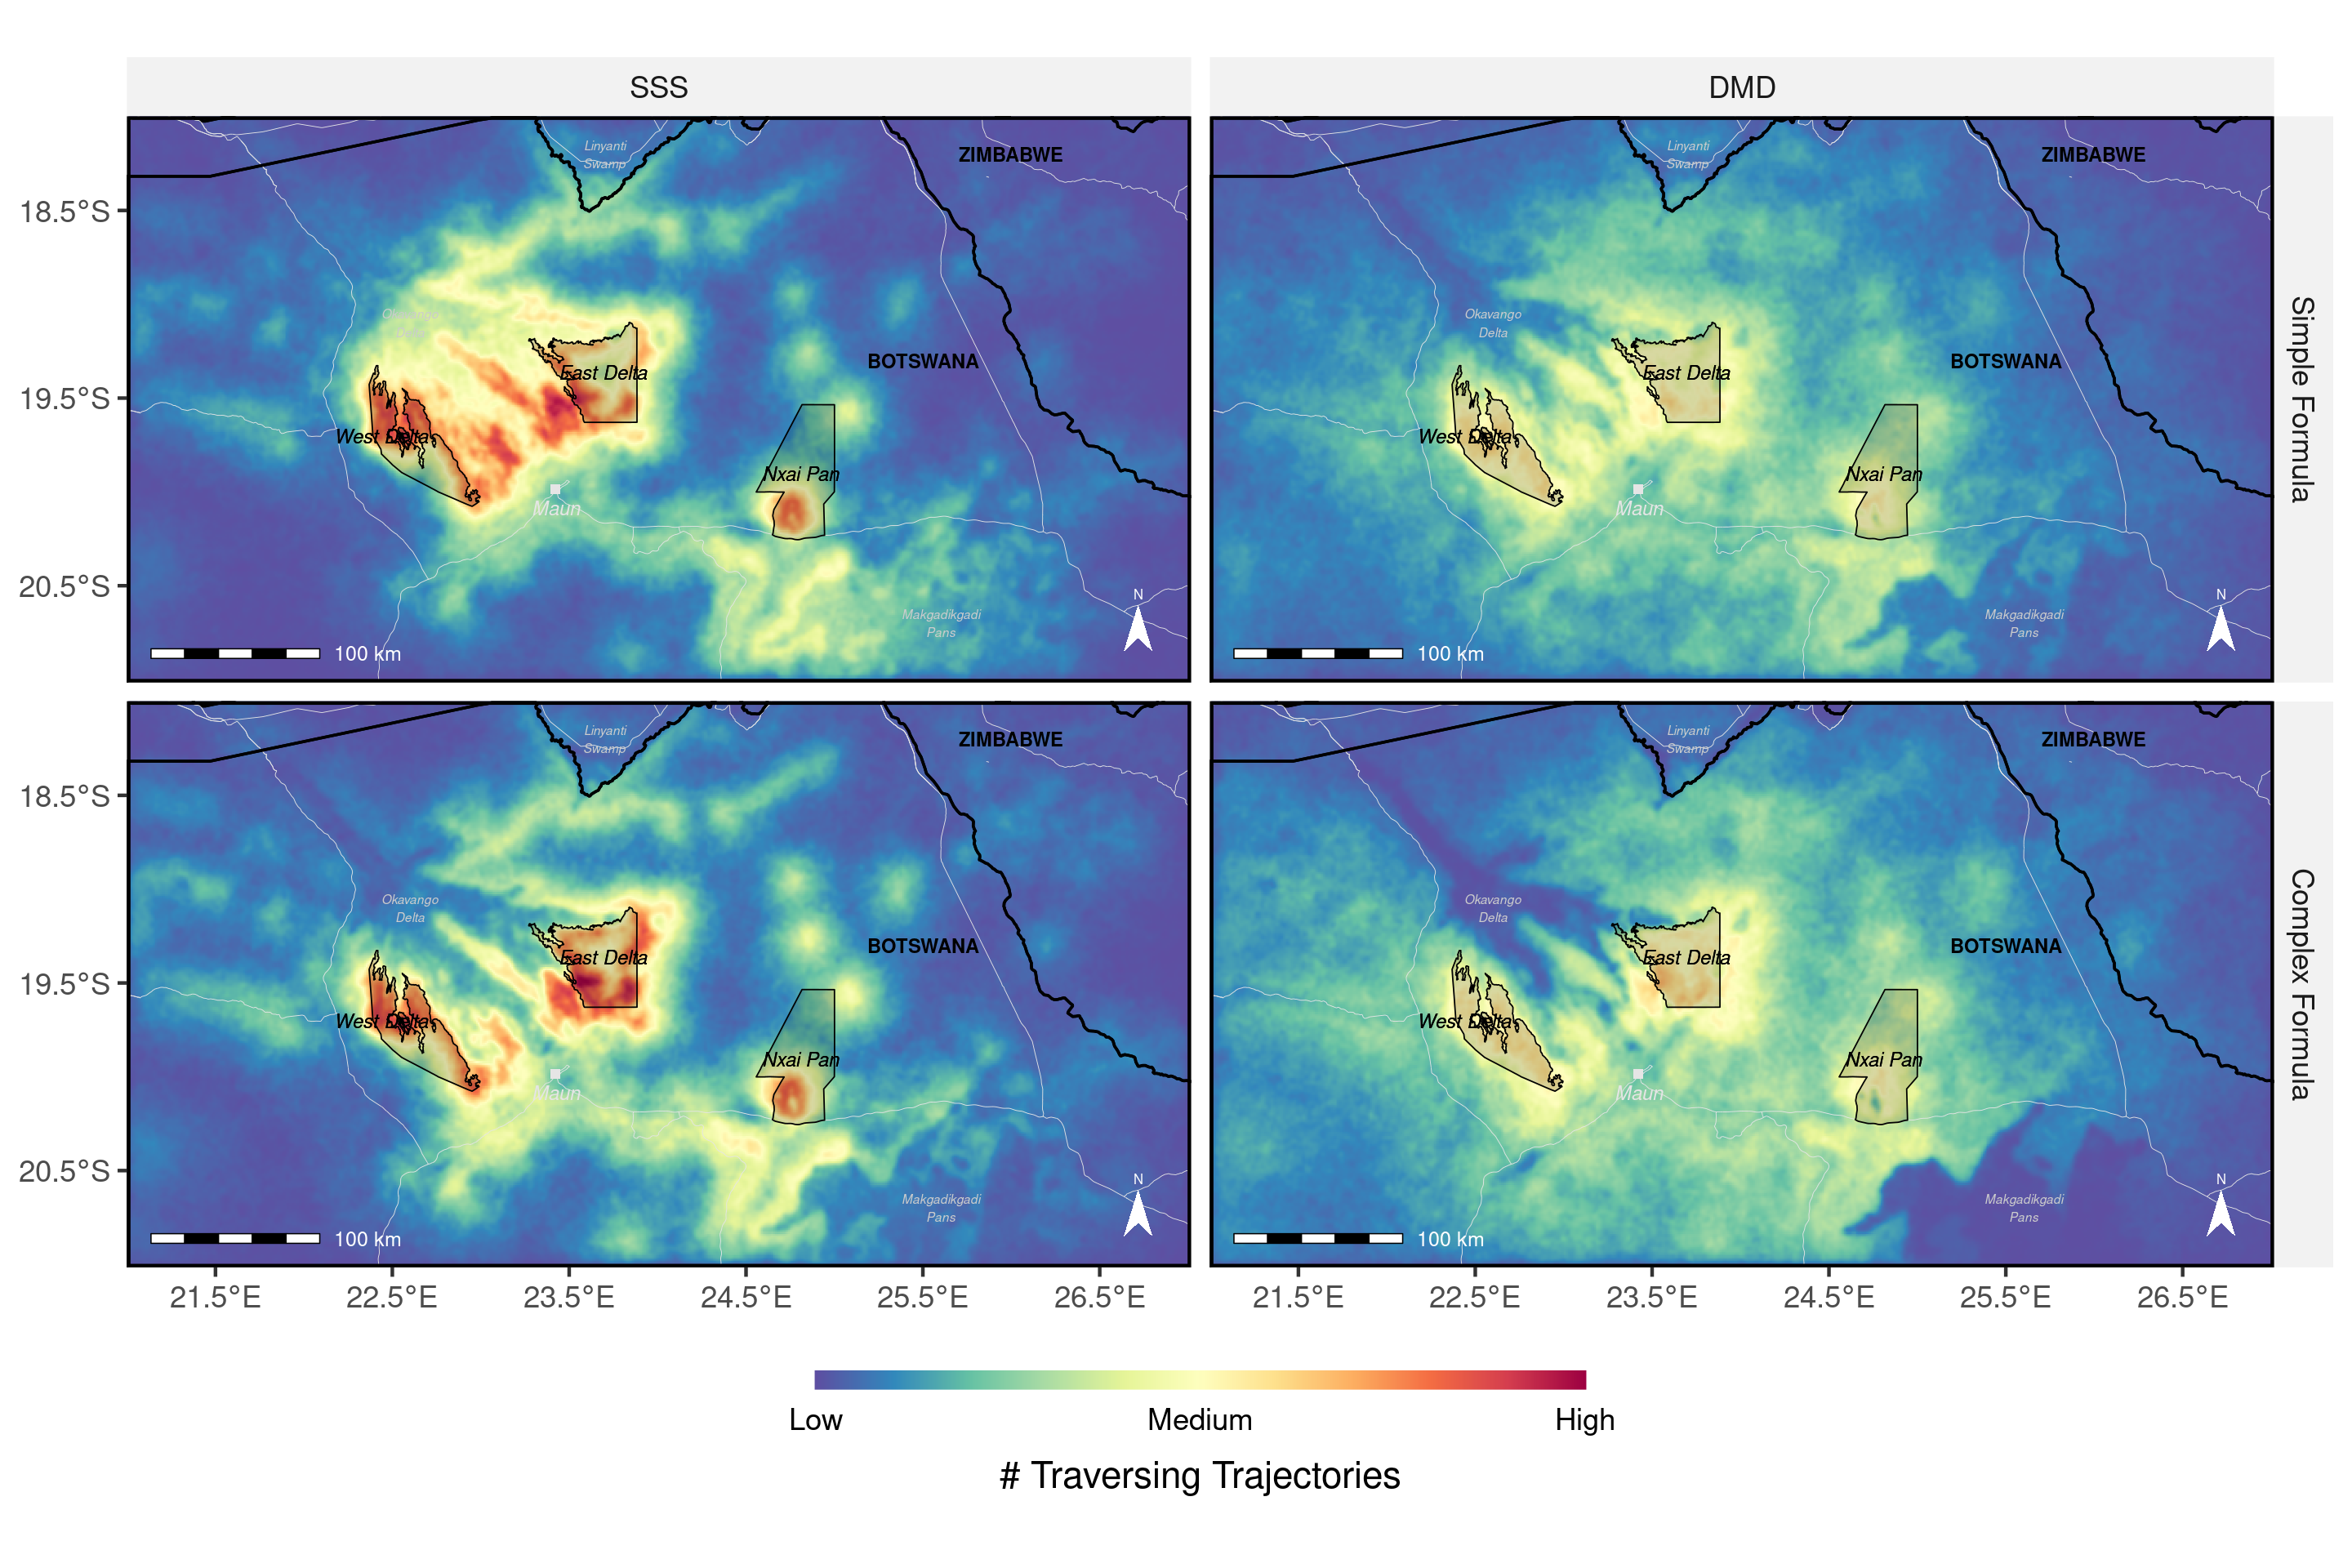
\includegraphics[width = \textwidth]{Figures/HeatmapComparison}
  \caption{Heatmaps derived under the most static (SSS) and dynamic (DMD)
  configurations. Results are shown for both the simple and full model.}
  \label{HeatmapComparison}
 \end{center}
\end{figure}

\section{Discussion}

\subsection{Brief Summary}

We introduced a framework to highlight that seasonality can enter a connectivity
analysis at three distinct stages; (1) when extracting spatial covariates for
fitting the selection model, (2) when fitting the selection model, and (3) when
predicting from the fitted model. Through combination, this yields six
configurations that differ in their degree of dynamism and, arguably, realism.
We fitted the models associated with each configuration using GPS data on
dispersing wild dogs and iSSFs and employed a rigorous validation procedure to
investigate potential gains in predictive performance that can be reaped by
incorporating different levels of dynamism. Results from the fitted models
showed that including seasonality only marginally affected the inferred patterns
of habitat selection and movement behavior. Similarly, the validation procedure
suggested only moderate improvements in predictive performance upon increasing
the degree of dynamism. Crucially, these benefits were limited to an overly
simplistic model and vanished upon fitting a more complex one. We therefore
could not pinpoint a specific stage at which including seasonality was
particularly beneficial. Despite this, we found that dispersal simulations under
the most static and most dynamic configurations resulted in differing
connectivity patterns. Under the most static configuration, landscape
connectivity was clumped around a few hot spots, whereas it was homogeneously
distributed across the landscape under the most dynamic configuration. Finally,
our work demonstrated that simulations from IBMMs effectively allow rendering
seasonal changes in the landscape, achieving a degree of seasonal dynamism and
realism that cannot be reached using permeability-based connectivity models.

\subsection{Moderate Improvements upon Increasing Dynamism}

Our validation procedure revealed only moderate improvements in our ability to
predict dispersal movements when increasing the degree of dynamism. Given the
system's extreme seasonal variability, this was somewhat surprising. We believe
that the absence of a more pronounced improvement can be traced back to multiple
factors. Firstly, we focused our analysis on dispersing individuals, which cover
large distances in search of potential mates and a suitable territory
\citep{McNutt.1996, Cozzi.2020}. In our case, the average 4-hourly step length
was 2.5 km, suggesting that dispersers cross and sample numerous unfamiliar
areas and potentially unsuitable habitats within short time. We thus hypothesize
that the spatial scale at which seasonality affects environmental
characteristics did not suffice to match the spatial scale at which our focal
species perceives and moves across the landscape during dispersal. A Further
explanation could be that dispersing individuals prioritize finding unoccupied
territories or areas with low competition, rather than focusing on specific
habitat types (e.g., \citealp{Creel.1996, Creel.2001}). Dispersers' habitat
selection may therefore be more strongly influenced by territorial
considerations (sensu \citealp{Cozzi.2018}) and only little affected by
seasonally changing landscape characteristics. This would also explain the
relatively weak selection or avoidance of environmental characteristics
exhibited in \Cref{MovementModel}. Finally, the AWD is a generalist species that
can occupy a broad variety of habitats \citep{Woodroffe.2011}. A certain
tolerance towards changing environmental conditions can therefore be expected
and may explain why seasonal differences were faint. This holds particularly
true for dispersers, which are usually more tolerant towards unfavorable habitat
conditions as they spend little time within the same area \citep{ONeill.2020}.

\subsection{Substantial Improvements upon Fitting a Complex Model}

In comparison to the improvements achieved by increasing dynamism, a more
significant improvement in predictive ability was achieved by moving from the
simple to the full iSSF model. In the full model, we included several
interactions that accounted for wild dogs' biology, such as reduced movement
during dark nights \citep{Cozzi.2013} or during times of high ambient
temperature \citep{Rabaiotti.2021}. Even though these interactions are not
directly linked to connectivity, they clearly accounted for a substantial amount
of variation in observed dispersal movements and facilitated predictions from
the fitted model. We also allowed for potential changes in dispersers' movement
behavior depending on habitat conditions, such as shorter steps in areas covered
by water \citep{Hofmann.2023}. Overall, the inclusion of these interactions
elevated the predictive ability of our dispersal model to such a high level that
increasing dynamism did not provide any further improvements. Notably, the
ability of encapsulating such a detailed and mechanistic understanding of
dispersal movements is unique to IBMMs and cannot be achieved using
permeability-based connectivity models.

\subsection{Dynamic Connectivity}

When comparing connectivity under the most static (SSS) and dynamic (DMD)
configurations, we observed that connectivity was clumped along a few major
dispersal hotspots under the static configuration, but homogeneously distributed
across the entire landscape under the dynamic configuration. This corroborates
previous research showing that static representations tend to result in an
underestimation of connectivity because seasonal stepping stones or corridors
are missed \citep{Martensen.2017}. With the help of such seasonally-available
dispersal habitats, areas that would otherwise be difficult to reach become
accessible, even if only for a limited time. In our study, such stepping stones
could arise in two ways. Firstly, the landscape could change seasonally, which
may have shifted preferred habitats, leading to the emergence of alternative
movement corridors. In addition, habitat or movement preferences of simulated
individuals could change, resulting in different habitat characteristics being
traversed depending on the season. In combination, varying landscape conditions
and species preferences resulted in a more balanced mosaic of connectivity
across the year. Importantly, the fact that connectivity is more evenly
distributed across the year does not exclude the possibility that certain areas
experience lower connectivity seasonally. As already shown by
\citet{Osipova.2019}, a static representation may result in both an over- and
under-estimation of short-term connectivity, depending on the area and season.
For conservation planning, this implies a need to protect landscapes at broader
scales, as areas that provide little connectivity during some season may become
critical during others. A dynamic take at connectivity therefore improves our
understanding of ecological processes in dynamic landscapes and may help to
identify otherwise overlooked dispersal hotspots.

\subsection{The Costs of Incorporating Dynamism}

Increasing seasonal dynamism to model dynamic connectivity comes at significant
costs, both in terms of data requirements and computational challenges. To
represent seasonal changes in the landscape, one needs to download and process
frequently updated spatial layers for each seasonal covariate. This is
time-consuming and implies a substantial increase in the data-volume that needs
to be handled. Because seasonal products are comparably rare, the choice to
model connectivity dynamically will also entail a significant restriction in the
number of potential covariates or require custom remote sensing algorithms
(e.g., Appendix A1). Seasonal or remote sensed layers are also more susceptible
to noise and missing values, particularly in cases where cloud cover is
frequent. Extracting covariates from seasonal layers poses a further challenge,
as data need to be extracted from those layers that best represent environmental
conditions at the time of the respective observed or random step. This applies
to the extraction of data for model fitting, as well as when extracting data
during the simulation. Finally, splitting the species data by season to fit
seasonal selection models significantly reduces the amount of data remaining per
season, potentially causing convergence issues. In our case, these additional
efforts were not outweighed by an improved predictive ability. This finding is,
however, likely highly specific to our study system. We therefore do not wish to
discourage future studies from accounting for seasonality when assessing
connectivity. Instead, we'd like to view our study as an example that the
benefits of increased realism do not necessarily justify the additional
complexity they bring about and that the associated costs and benefits need to
be carefully pondered \citep{Puy.2022}.

\subsection{Validation Procedure}

Our validation procedure was focused on validation at the step level, but did
not directly test how well predictions of functional connectivity agreed with
true connectivity. This was owed to a conceptual limitation when trying to
validate seasonal connectivity predicted from an IBMM. In seasonal landscapes,
connectivity not only varies spatially, but also temporally. A meaningful
validation therefore requires that connectivity is predicted separately for each
timestamp in the validation data. In our case, for instance, the fact that the
landscape was updated every 4 hours implies that a new connectivity map would
need to be created around each validation step. This is equivalent to validating
connectivity at the step level, which is why we deemed the application of k-fold
cross-validation for case and control studies using Spearman's rank correlation
as an appropriate validation technique. Note, however, that Spearman's rank
correlation coefficient is heavily dependent on the number of steps per stratum
and should therefore not be used to compare predictive efficacy across studies
(Figure S11). For static connectivity analyses, alternative validation
techniques exist. \citet{McClure.2016}, for instance, proposed a suite of
validation metrics (applied in \citealp{Zeller.2018, Finerty.2023}). These
largely work by comparing connectivity at random locations with connectivity at
locations where the focal species was observed. Because these metrics fail to
account for potential autocorrelation in the validation data (which is usually
present in GPS data; \citep{Otis.1999}), \citet{Brennan.2020} suggested
validating connectivity by applying a path- or step-selection model to withheld
data. If the fitted model proves significant selection towards areas of high
connectivity, predictions are indeed indicative of functional connectivity
(sensu \citealp{Brennan.2020}). Developing similar approaches for dynamic
connectivity analyses remains a task for future studies.

\subsection{Seasonal Habitat Selection}

% In the Okavango Delta, water is among the most temporally variable landscape
% features that drives the distribution of species over large spatial scales
% \citep{McCarthy.1998, Ramberg.2006, Bartlam-Brooks.2011, Bennitt.2014}. Wild
% dogs, like most other large carnivores, may avoid a large distance to water
% because of prey-availability in its vicinity \citep{Redfern.2003, Bonyongo.2005,
% Valeix.2010}. At the same time, wild dogs are terrestrial mammals and avoid
% crossing water \citep{Cozzi.2013}, even during dispersal \citep{Hofmann.2021}.

When we fit models assuming static covariates, wild dogs displayed a preference
for areas close to water, irrespective of the season. However, water itself
appeared to be only avoided during the dry season. This was likely caused by a
misrepresentation of areas covered by water in the static configuration. Since
rainwater collected in Angola only slowly descents through the Okavango Delta's
tributaries \citep{McCarthy.1997}, large portions of its floodplains remain dry
during the wet season \cite{McCarthy.2003}. On static covariates, which
represent average conditions across both seasons, it may appear as if
individuals moved through areas covered by water, albeit in reality they likely
moved along them. Indeed, upon accounting for such seasonal changes by
considering seasonally updated covariate layers, parameter estimates from the
selection models assimilated and suggested avoidance of water across both
seasons. Our choice of splitting data into wet and dry season based on a fixed
set of dates can be viewed as a further limitation, as it assumes an immediate
switch from one season to another. In reality, season-transitions are not abrupt
but rather gradual and their timing may vary from year to year. A more robust
approach would therefore be to define the start and end of each season based on
bio-climatic descriptors and to ignore data collected during transitional
periods. This may imply a loss of data, but could help to detect seasonal
selection patterns. In our case, retaining all data was necessary to ensure
model convergence, but may have resulted in a cross-contamination between
seasons and therefore reduced our ability to pick up seasonal differences in
parameter estimates. Indeed, other studies reported that habitat selection of
their focal species varied greatly between seasons (but see
\citealp{Squires.2013}). \citet{Benz.2016}, for instance, found that dispersing
in elk (\textit{Cervus elaphus}) exhibit vastly different habitat preferences
during winter and summer. Similarly, \citet{Osipova.2019} report that habitat
selection of African elephants (\textit{Loxodonta africana}) in South Africa
differs between the wet and dry season. The importance of seasonality thus
appears to be highly system dependent.

% In cases where animals move along borders of two types of habitats
% that shift seasonally, a seasonal representation of habitat conditions seems
% paramount to prevent misleading conclusions.

% Other studies, however, report consistent preferences, irrespective of the
% season. \citet{Squires.2013}, for instance, show that habitat selection by lynx
% (\textit{Lynx lynx}) only differs little between winter and summer. Notably, the
% authors find that inferred patterns of connectivity were similar across seasons.
% However, few of them accounted for seasonality in their covariates, so it is not
% clear whether differences were are truly indicative of a behavioral changes or
% simply reflect changes in environmental conditions.

\subsection{Conclusion}

In conclusion, we explored the importance of incorporating different degrees of
dynamism when studying dispersal and connectivity. Overall, our findings
suggested only moderate improvements in predictive performance upon increasing
the level of dynamism. Nevertheless, connectivity patterns as inferred from
simulated dispersal trajectories differed vastly, with connectivity being more
evenly distributed when seasonality was accounted for. While increased realism
via improved representation of seasonality may offer novel insights into
ecological processes, the benefits must be carefully weighed against the added
complexity and effort required to collect seasonal data and model seasonal
dynamism in the focal species' preferences. Moving forward, our study serves as
an example that while accounting for seasonality could be crucial for some study
systems, it may not always justify the additional complexity, emphasizing the
need for thoughtful consideration of costs and benefits in future research.

\section{Authors' Contributions}

D.D.H. and G.C. conceived the study and designed methodology; D.D.H., G.C.,
D.M.B, and J.W.M. collected the data; D.D.H. analysed the data; G.C. assisted
with modeling; D.D.H. and G.C. wrote the first draft of the manuscript and all
authors contributed to the drafts at several stages and gave final approval for
publication.

\section{Data Availability}

Access to R-scripts to replicate our analyses will be provided through an online
repository at the time of publication.

\section{Acknowledgments \& Funding}

We thank the Ministry of Environment and Tourism and the Department of Wildlife
and National Parks of Botswana for granting permission to conduct this
research. D.D.H. was funded by a Swiss National Science Foundation Grant No.
310030\_204478 to G.C.

\newpage
\begingroup
\singlespacing
\ifthenelse{\boolean{usebiblatex}}{
  \begin{refcontext}[sorting=nyt]
  \printbibliography
  \end{refcontext}
}{
  \bibliography{LiteratureBibtex}
}
\endgroup

\end{document}
